\documentclass[11pt,noabs]{starlink}

% -----------------------------------------------------------------------------
% ? Document identification
\stardoccategory    {Starlink Cookbook}
\stardocinitials    {SC}
\stardocsource      {sc1.2}
\stardocnumber      {1.2}
\stardocauthors     {H.\,Meyerdierks, D.\,Ward-Thompson}
\stardocdate        {10 November 1995}
\stardoctitle       {JCMTDR Cookbook}
\startitlepic{
\begin{center}
\vskip -30mm
\leavevmode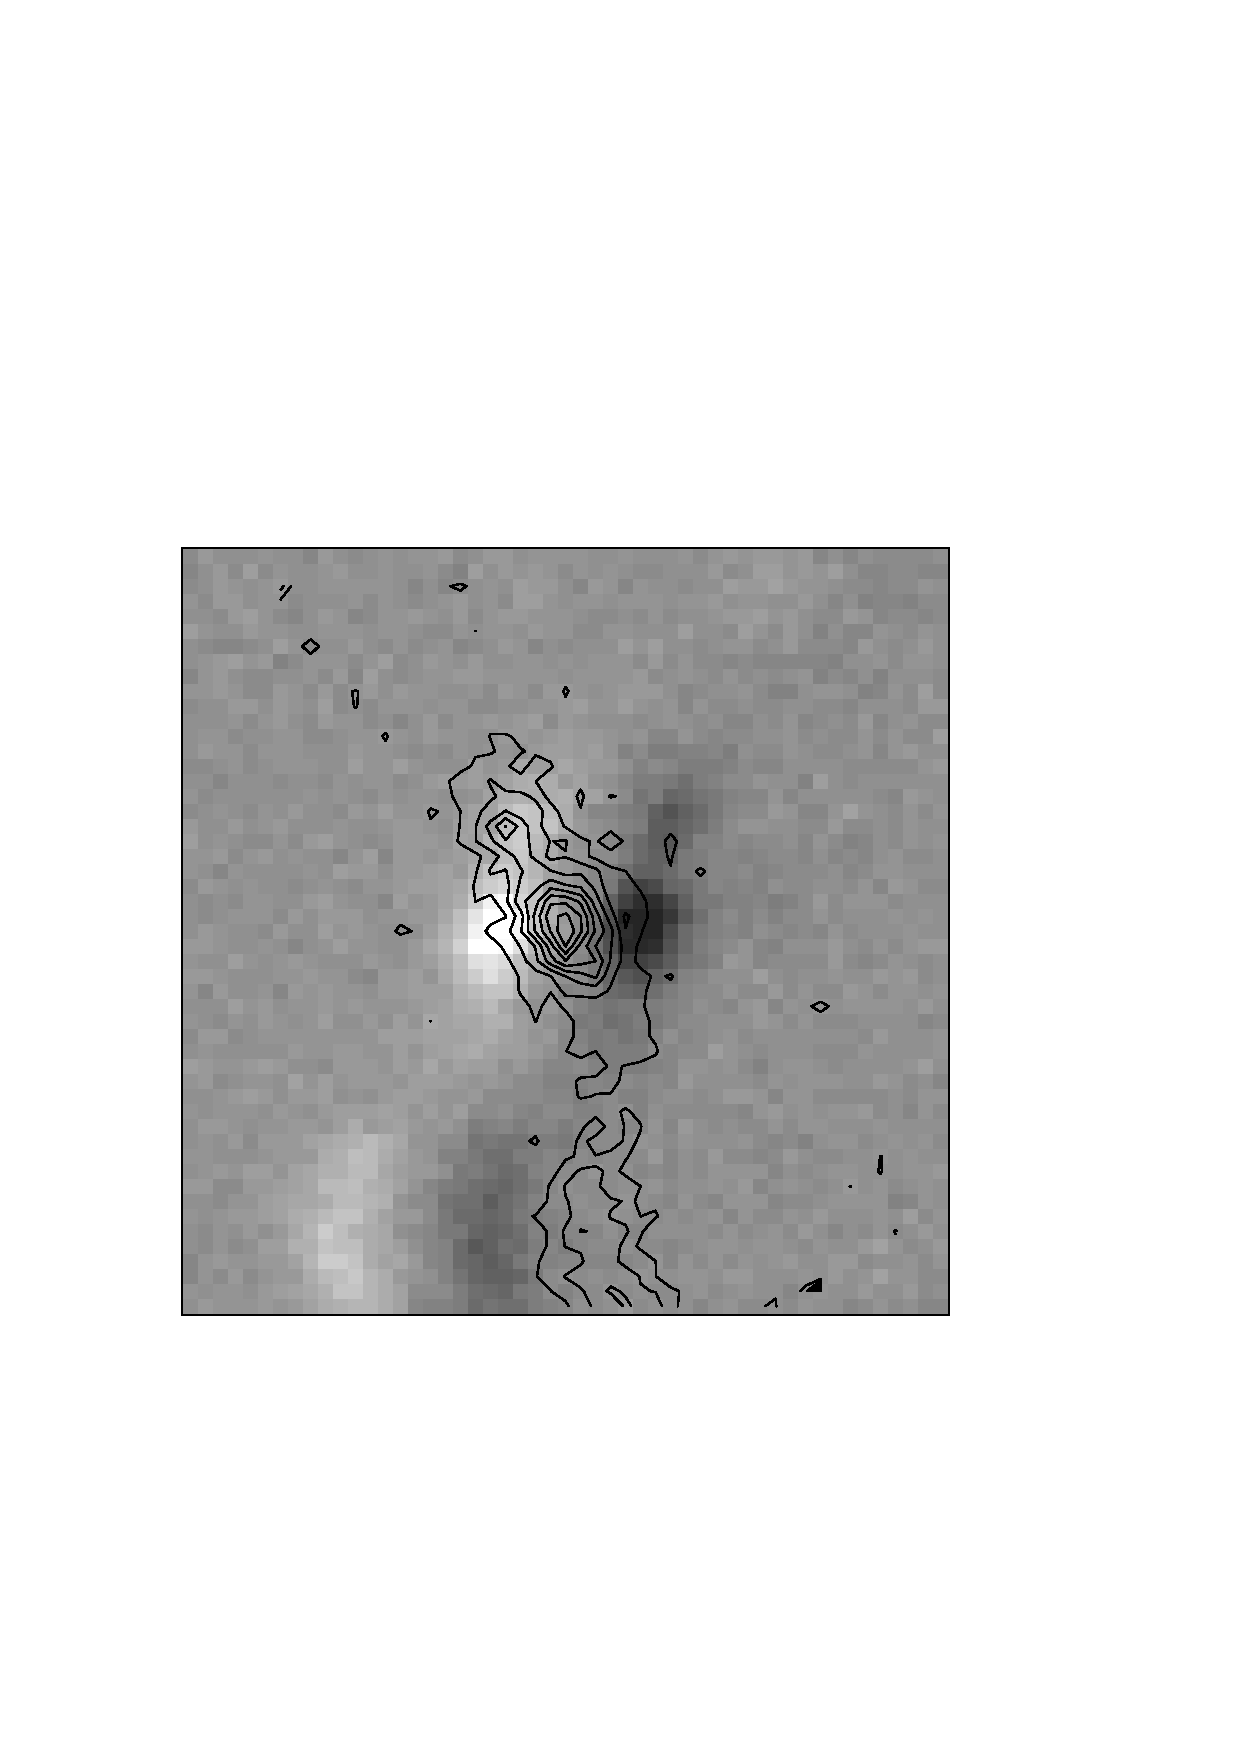
\includegraphics[height=120mm]{sc1_cover}

Grey: JCMT double-beam map in azimuth/elevation\\
Contours: The same map restored to single beam\\
and transformed to right ascension/declination
\end{center}
}
% ? End of document identification
% -----------------------------------------------------------------------------
% ? Document specific \providecommand or \newenvironment commands.
\providecommand{\htmltex}[1]{}
% ? End of document specific commands
% -----------------------------------------------------------------------------
%  Title Page.
%  ===========
\begin{document}
\scfrontmatter

\section{\label{roadmap}\xlabel{roadmap}Road map}



   When studying this document you may not want to read all sections,
   and it may not be sensible to read them in sequence. The following
   map gives you a two-dimensional representation of the contents, with
   suitable routes marked in different colours. You can use the map to
   visit each section and return here between sections. You can
   also use the navigation signs at the bottom of each section to
   get to the next section on the standard route, or to take detours.
   Many of the technical terms are explained in
Section~\ref{gloss}.

\begin{center}
\leavevmode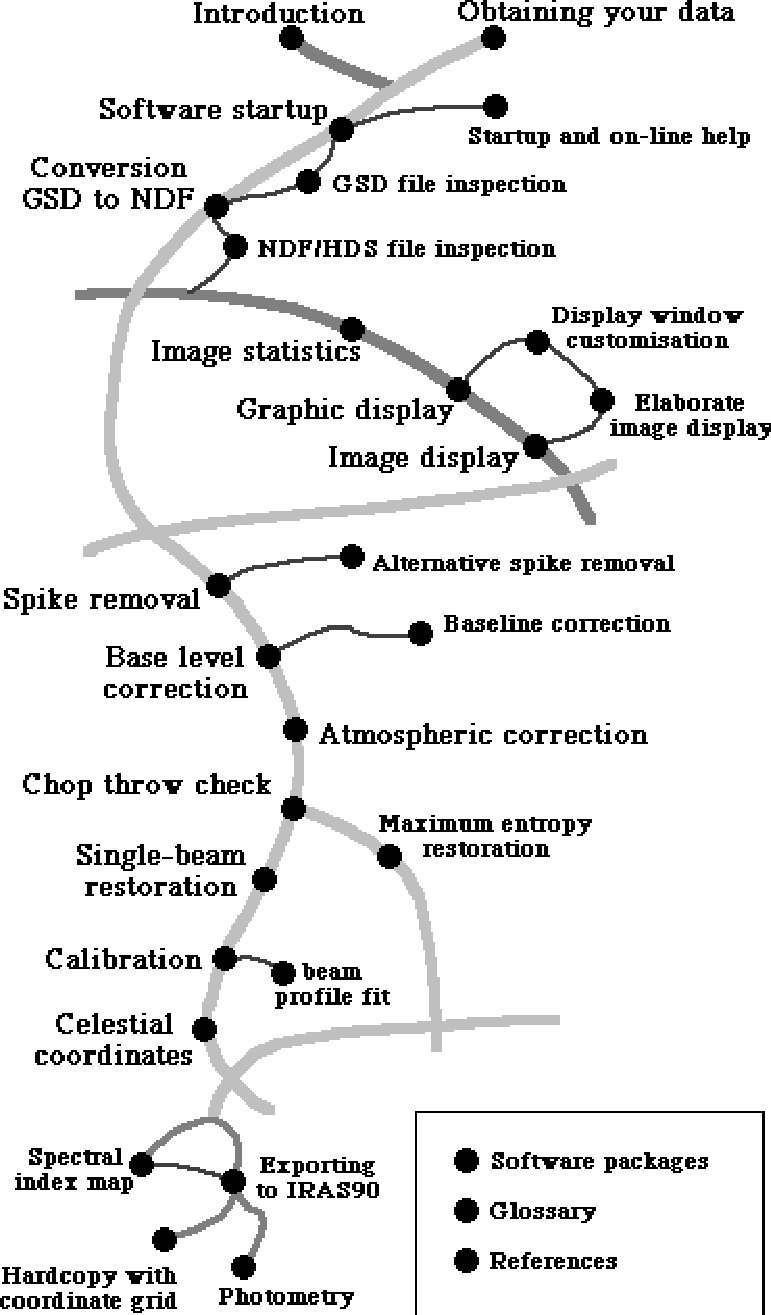
\includegraphics[height=150mm]{sc1_cont}
\end{center}

\section{\label{intro}\xlabel{intro}Introduction}

   This cookbook is intended for users of the
\htmladdnormallink{JCMT}{http://www.jach.hawaii.edu/JCMT/index.html}
   and its common-user bolometer UKT14
\htmlref{(Duncan et al. 1990).}{refer}
   It is intended as an introductory guide to the JCMT Data Reduction
   software package
\xref{(JCMTDR),}{sun132}{}
   which has been designed to replace the
\htmlref{NOD2}{glossnod2}
   software package for reduction of
\htmlref{dual-beam}{glossdualbeam}
\htmlref{on-the-fly}{glossonthefly}
   continuum maps. It is hoped that users who are new to the telescope
   as well as users already familiar with NOD2 will benefit from this
   cookbook. It tries to guide the user through the data reduction
   process and should be an aid to
   getting started in producing maps from raw dual-beam data.

   The central software package for the data reduction will be JCMTDR.
   However, this contains only the routines specific to this kind of
   data. More general reduction routines are
\htmlref{used from other software packages}{packs}
   in the
\htmladdnormallink{Starlink Software Collection.}{http://www.starlink.ac.uk/software.html}
   Each package offers
   more functions than described here and has its own extensive
   documentation.
   Users who regularly use the Starlink software will be familiar with
   many of the routines used here. Those who prefer other software,
   such as AIPS or IRAF, can use them, once the data have been
   calibrated and converted onto an RA/Dec grid, since the data
   can ultimately be put out in
\htmlref{FITS format.}{glossfits}

   We would like to thank John Lightfoot, Richard Prestage, and Kevin
   Richardson for providing useful comments on this document.


\section{\label{obtain}\xlabel{obtain}Obtaining your data}

   When taking the data there are many things which you can do to ensure
   that the quality of your data is as high as possible, and that it is
   possible to obtain the best calibration of your data. Firstly, it is
   important to know the atmospheric transmission at the time of your
   observations. This must be carefully monitored. The opacity at
   225 GHz is provided by the NRAO tipper radiometer, located at the
   nearby Caltech Sub-millimeter Observatory (CSO). This opacity, known
   colloquially as `cso-tau',
   gives the fractional zenith transmission \textit{exp(-tau)\/} at 225 GHz.
   Keep a record of the cso-tau throughout the period of your
   observations. The opacity at the frequency of your observations is
   related to the 225 GHz opacity by a series of empirical relations.
   The most common of these are cited in the astronomical literature
\htmlref{(Stevens \& Robson 1994;}{refer}
\htmlref{Sandell 1994),}{refer}
   but check with your support scientist during your observing run for
   the most up-to-date estimates of these relations.

   However, even tracking the cso-tau does not guarantee properly
   calibrated data. It is possible that the transmission in the
   direction of your source is different from that in the direction in
   which the cso-tau is measured. Therefore it is also necessary to
   obtain regular photometry throughout the night of a calibration
   source close to your target object. The best calibrators are the
   planets Uranus and Mars
\htmlref{(Griffin et al. 1986;}{refer}
\htmlref{Orton et al. 1986;}{refer}
\htmlref{Griffin \& Orton 1993),}{refer}
   although a number of secondary calibrators are now also catalogued
\htmlref{(Sandell 1994).}{refer}
   Preferably obtain calibration on more than one object. However,
   \emph{always\/} calibrate immediately before and after every
\htmlref{on-the-fly}{glossonthefly}
   map that you make, which gives you an additional handle on the
   variation of the opacity during the map. It is necessary to obtain
   calibration for
   at least one source a minimum of 3 times (preferably 5 or more) at
   all wavelength bands during the shift to allow a proper calibration
   of the data. Standard formulae can then be used to calculate the
   opacity at each wave-band in the direction of your source
\htmlref{(Sandell 1994).}{refer}
   The flux densities of the planets at the time of
   your observations can be
   found by running the JCMT utility programme \texttt{fluxes}. It is
   advisable to run this programme at the telescope to make sure you
   have the most up-to-date values for the planets' brightness
   temperatures. Obtain planet flux densities for each shift that you
   observe.

   If the night has been reasonably stable, and the sky relatively
\htmlref{photometric,}{glossphotometric}
   then the two methods should produce consistent results, and it should
   also be possible to calibrate
\htmlref{single-point photometry}{glosssinglepoint}
   data. In addition you must also make
\htmlref{beam maps}{glossbeammap}
   to calibrate your on-the-fly data. Beam maps are best made on planets
   which are compact relative to the beam, and reasonably bright. The
   best planets for this are Mars and Uranus. If no planet is available
   within your shift you could try compact secondary calibrators, or try
   to obtain beam maps outside of your shift. Consult with your support
   scientist if in doubt. In all cases you must make at least one, and
   preferably several, beam maps at every wavelength at which you have
   mapped target sources, using the same
\htmlref{chop throw}{glosschopthrow}
   and step size for the beam map as for the target object.

   There are a number of other tips which are worth bearing in mind,
   such as always over-sampling your maps. Since on-the-fly maps are
   made in azimuth/elevation coordinates and will later have to be
   converted to RA/Dec coordinates, a critically sampled map in
   Az/El may convert into an under-sampled map in RA/Dec. A
   rule of thumb is to make the map step size roughly one third of the
   diffraction limited beam size. Always make the length of the map rows
   longer than the width of the emitting source by \emph{twice\/} the chop
   throw. (Remember that the source will appear to rotate through the
   course of the night in the reference frame of the telescope.) This
   ensures that both beams of the dual beam map are off source at both
   ends of every row. Keeping the chop throw relatively small helps with
\htmlref{error beam}{glosserrorbeam}
   cancellation at high frequencies. Run the JCMT utilities
   \texttt{journal} and
   \texttt{usum} when at the telescope to obtain listings of all observations
   and maps made. This records important information such as the
\htmlref{sensitivity setting}{glosssensset}
   on which each map was made. Check with your support scientist before
   your run to make sure that you are aware of all the latest
   developments, such as the current dish surface accuracy.

\newpage
\section{Reduction}

\subsection{\label{start}\xlabel{start}Software startup}

   To make available all the applications (commands) used in this
   cookbook, do the following
\htmlref{package activations}{start2}
   for
\xref{Figaro,}{sun86}{}
\xref{Specdre,}{sun140}{}
\xref{IRAS90,}{sun163}{}
\xref{KAPPA,}{sun95}{}
   and
\xref{JCMTDR:}{sun132}{}

\begin{terminalv}
% figaro
% specdre
% iras90
% kappa
% jcmtdr
\end{terminalv}

   In this cookbook we make only minimal use of Figaro. If you are well
   accustomed to that package, you will notice that many tasks could be done
   with Figaro commands. If you are not familiar with it, we
   recommend that you learn the other packages instead.

\subsection{\label{gsd2ndf}\xlabel{gsd2ndf}Conversion GSD to NDF}

   Your raw data will be in the form of
\htmlref{`GSD' files,}{glossgsd}
   which is a JCMT-specific VAX-binary file format.
\texttt{\xref{makemap}{sun132}{MAKEMAP}}
   reads the data and observation description from a JCMT GSD file and
   can put it out in the standard Starlink
\htmlref{NDF format,}{glossndf}
   readable by
\xref{KAPPA}{sun95}{}
   and
\xref{Figaro.}{sun86}{}

   It is recommended that NDF is chosen as the preferred Figaro format
   so that \texttt{makemap} will create NDF format rather than the older
\htmlref{DST format.}{glossdst}
   If you check your
   environment variable FIGARO\_FORMATS it will probably be all right:

\begin{terminalv}
% echo $FIGARO_FORMATS
ndf,dst
\end{terminalv}
% This comment provides a $ matching the verbatim one so that colour
% highlighting in emacs does not get too upset.

   If `dst' is the first or only choice, then you have to change this:

\begin{terminalv}
% setenv FIGARO_FORMATS ndf,dst
\end{terminalv}

   Then you can run \texttt{makemap} on the GSD file:

\begin{terminalv}
% makemap gsdfile=rxa_146.dat output=rxa_146m tel_beam=M pos_beam=R
\end{terminalv}

   Note that the output file has a `file name extension' of `.sdf' for
\htmlref{`Starlink Data File',}{glosssdf}
   also known as
\htmlref{`HDS file'.}{glosshds}
   That is to say, the file we created is called \texttt{rxa\_146m.sdf}.
   With Starlink applications you must never give the file name
   extension, only the stem of the file name. When you talk to the
   computer's operating system about the file, then you have to give the
   full file name, of course.

\subsection{\label{stats}\xlabel{stats}Image statistics}

   The statistics of an image can be examined at any stage of the
   reduction with the command
\texttt{\xref{stats:}{sun95}{STATS}}

\begin{terminalv}
% stats rxa_146m

  Pixel statistics for the NDF structure /tmp_mnt/home/hme/dump/rxa_146m

     Title                     : OMC1
     NDF array analysed        : DATA

        Pixel sum              : 21094.68
        Pixel mean             : 5.212425
        Standard deviation     : 0.464714
        Minimum pixel value    : 1.335313
           At pixel            : (41, 29)
           Co-ordinate         : (20, 0)
        Maximum pixel value    : 9.292433
           At pixel            : (31, 29)
           Co-ordinate         : (-20, 0)
        Total number of pixels : 4047
        Number of pixels used  : 4047 (100.0%)
\end{terminalv}

\subsection{\label{idset}\xlabel{idset}Graphic display}

   Assuming that you use an X screen, prepare your display with the commands
\texttt{\xref{gdset}{sun95}{GDSET}},
\texttt{\xref{idset}{sun239}{IDSET}},
\texttt{\xref{lutgrey}{sun95}{LUTGREY}},
   and
\texttt{\xref{paldef}{sun95}{PALDEF}}.

\begin{terminalv}
% setenv DISPLAY myscreen.here.ac.uk:0
% gdset xw
% idset xw
% lutgrey
% paldef
\end{terminalv}

   See also
Section~\ref{xmake}
   for more detailed information
   about controlling the display window characteristics.

\subsection{\label{display}\xlabel{display}Image display}


   At any point in the data reduction you can examine the image
   by displaying it with
\texttt{\xref{display}{sun95}{DISPLAY}}.
   If you want more than a very simple grey-scale
   display, see
Section~\ref{display2}
   for more detailed information.
   After the
\htmlref{graphics device has been set up}{idset}
   properly, we can display the map:

\begin{terminalv}
% display in=rxa_146m mode=scale accept
\end{terminalv}

\begin{center}
\leavevmode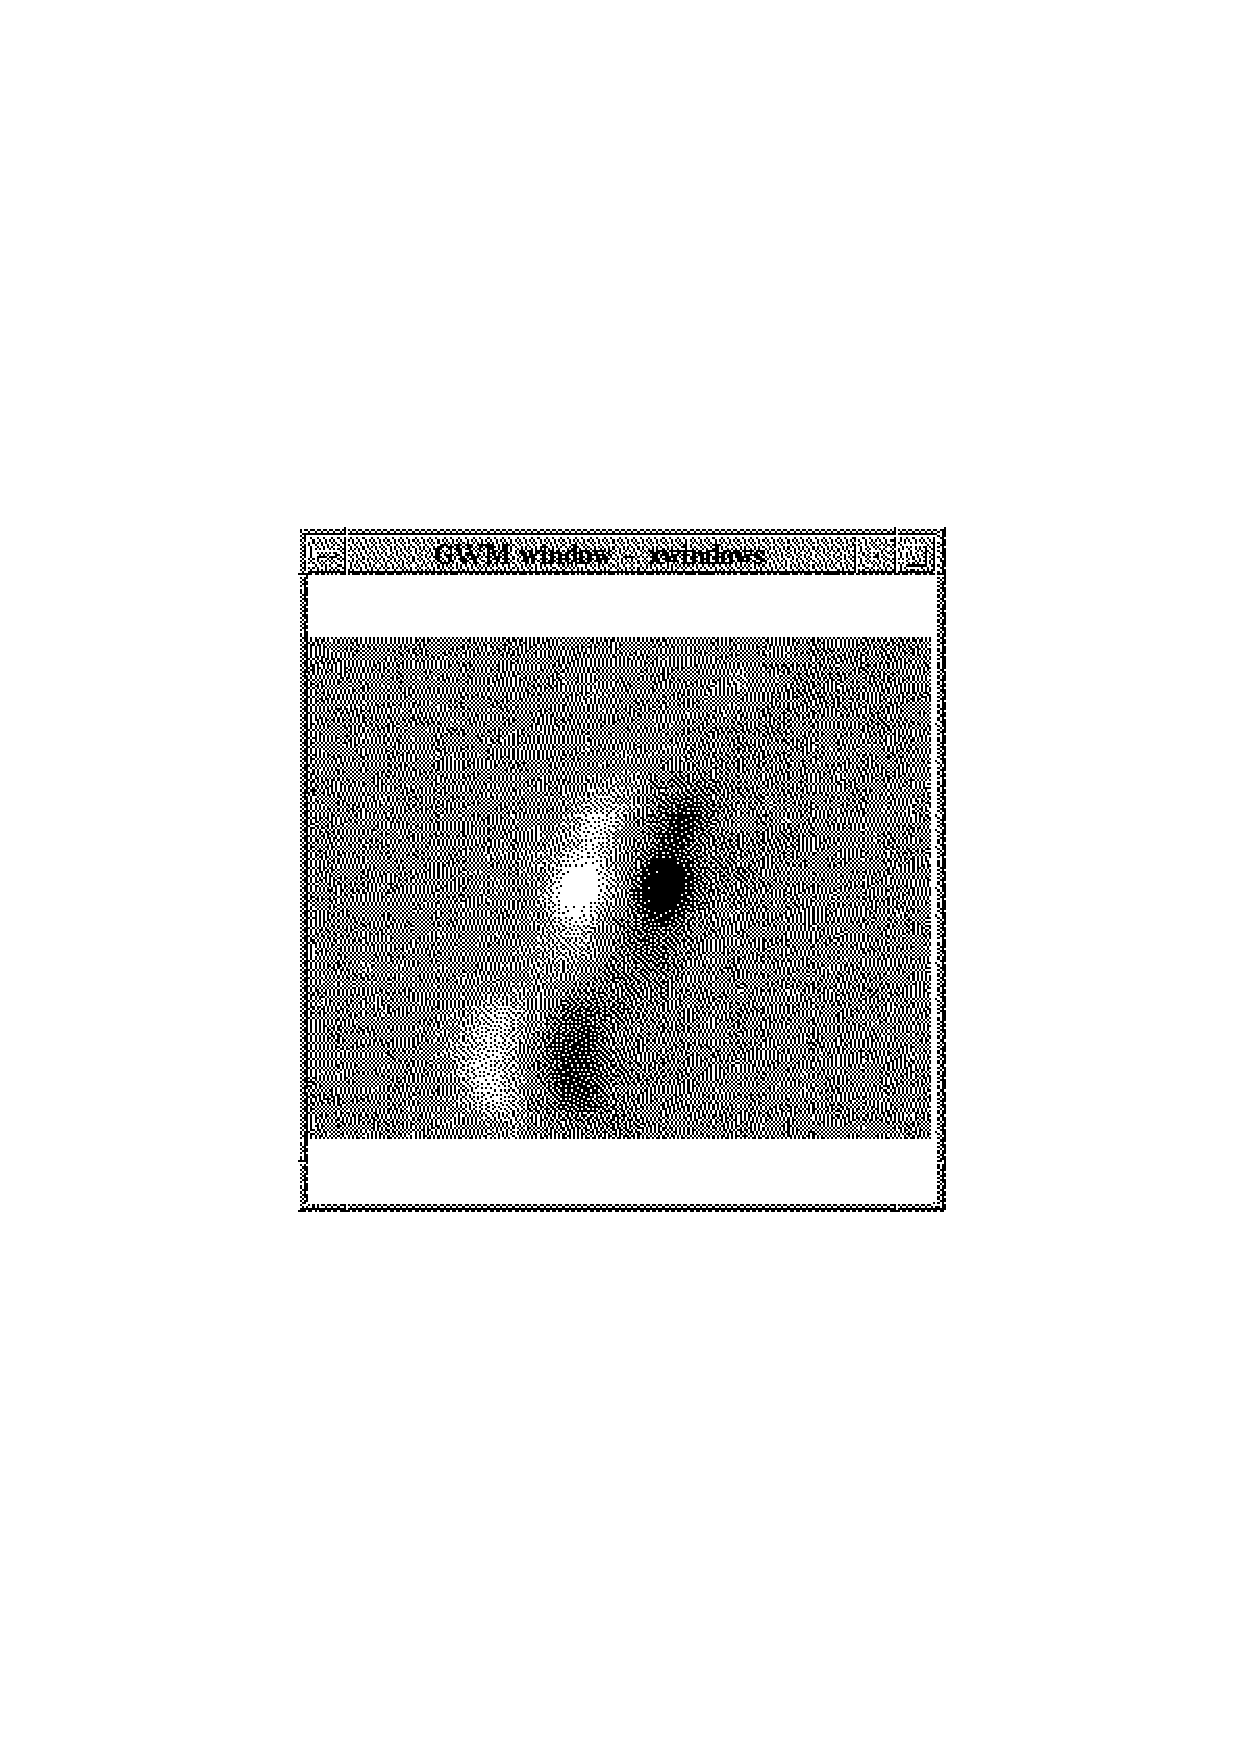
\includegraphics[height=80mm]{sc1_display1}
\end{center}

\subsection{\label{spikes}\xlabel{spikes}Spike removal}



   The next task after converting the data to NDF format
   is to remove spikes from the data. This can usually
   be carried out using the routine
\texttt{\xref{zaplin}{sun95}{ZAPLIN}}.
   See
Section~\ref{spikes2}
   if you have to remove spikes by interpolation within the row and
   ignoring the rows below and above the spike.

   In the following example two individual pixels are replaced with an
   interpolation of their neighbourhood. Work on individual pixels is
   achieved by selecting the pixel as both corner points of a region.
   The endless loop asking for the next zapping action is broken by
   giving the so-called
\htmlref{null value,}{glossnullvalue}
   an exclamation mark. You can also
   replace a whole row (or column) by giving `lines' (`columns') as
   value for \texttt{lincol}. The display is not updated during
   \texttt{zaplin}, you
   have to
\texttt{\xref{display}{sun95}{DISPLAY}}
   the output afterwards, if you want to check.

\begin{terminalv}
% display in=rxa_146m accept
% zaplin mode=cursor zaptype=linear out=rxa_146mc

Type a 1 or a space to select a point.
Type . to exit.

LINCOL - Lines, Columns or Region? /'LINES'/ > region
Use the cursor to select 2 points.
Zapping region ( 17, 47 ) to ( 17, 47 ).

LINCOL - Lines, Columns or Region? /'REGION'/ >
Use the cursor to select 2 points.
Zapping region ( 25, 47 ) to ( 25, 47 ).

LINCOL - Lines, Columns or Region? /'REGION'/ > !
\end{terminalv}

   \texttt{zaplin} interpolates using the nearest neighbours in the image,
   it takes into account neighbours in the previous and next rows as well
   as in the same row as the zapped pixel.
   Caution should be exercised when removing apparent
   `spikes' from source regions.

\subsection{\label{base}\xlabel{base}Base level correction}

   The
\htmlref{on-the-fly maps}{glossonthefly}
   all have an arbitrary constant of around +5 mV
   added to them, such that both positive and negative beams can be
   accommodated within the range of the detector. This constant must be
   subtracted off next. For simple sources with circular geometries, and
   symmetric maps (e.g.\ planets), where the bolometer has remained
   stable throughout the period of the map, it is possible to just take
   the average value for the whole image. This is found using
\texttt{\xref{stats}{sun95}{STATS}}.
   It is then subtracted from the whole image using
\texttt{\xref{csub}{sun95}{CSUB}}.
   Then perform the statistics again to check that this
   has worked:

\begin{terminalv}
% stats ndf=rxa_146mc | grep 'Pixel mean'
        Pixel mean             : 5.212425
% csub in=rxa_146mc scalar=5.212425 out=rxa_146mcs
% stats accept

  Pixel statistics for the NDF structure /home/mydir/data/rxa_146mcs

     Title                     : KAPPA - Csub
     NDF array analysed        : DATA

        Pixel sum              : -0.001919
        Pixel mean             : -4.74245E-7
        Standard deviation     : 0.464714
        Minimum pixel value    : -3.877112
           At pixel            : (41, 29)
           Co-ordinate         : (20, 0)
        Maximum pixel value    : 4.080008
           At pixel            : (31, 29)
           Co-ordinate         : (-20, 0)
        Total number of pixels : 4047
        Number of pixels used  : 4047 (100.0%)
\end{terminalv}



   For more complex sources, it is best
   to subtract a different constant from each row (if the baseline has
   drifted, then a straight line should be subtracted), determined from
   the ends of each row, in the region where both beams were `off source'.
   See
Section~\ref{base2}.

\subsection{\label{extinct}\xlabel{extinct}Atmospheric correction}

   The next step of the process is to take out the effect of the
   atmosphere. This is carried out using the routine
\texttt{\xref{jcmtextc}{sun132}{JCMTEXTC}}.
   This application corrects JCMT data for the effect of atmospheric
   extinction. The air mass at which each map pixel was observed is
   calculated, and multiplied by the estimated zenith atmospheric
   extinction at the time of observation to give the extinction optical
   depth along the line of sight. Multiplying the data point by the
   exponential of the optical depth gives the value that would have been
   measured above the atmosphere.



   The zenith optical depth is assumed to
   vary linearly with time between the values given by the parameters
   \texttt{tau} and \texttt{endtau}. These parameters must be
   given by the user, having calculated them using the methods outlined
   in
Section~\ref{obtain}.

\begin{terminalv}
% jcmtextc input=rxa_146mcs output=rxa_146mcse tau=1.36 endtau=1.32
\end{terminalv}


\subsection{\label{throwchk}\xlabel{throwchk}Chop throw check}

   Before we proceed any further, we should check that the actual
\htmlref{chop throw}{glosschopthrow}
   is exactly the requested value. The requested throw is stored with
   the data, but it may have to be corrected to reflect the actual
   chop throw as determined from the
\htmlref{beam maps.}{glossbeammap}
   To determine the actual chop throw use the application
\texttt{\xref{fitgauss}{sun140}{FITGAUSS}}
   on the row of your beam map that goes through the centre of the
   planet. Fit two Gaussian profiles, one positive, one negative and
   work out the distance between the fitted centres. The
\texttt{\xref{editext}{sun140}{EDITEXT}}
   command is just to remove the data extension that \texttt{fitgauss}
   creates.

\begin{terminalv}
% fitgauss in=planet1\(,29\) mask1=-500 mask2=500 comp=\[1,2\] \
 ncomp=2 cont=0 centre=\[-20,20\] peak=\[5,-5\] fwhm=\[10,10\] \
 device=xw accept
...
Gauss components:
 #   centre pos.    peak height       FWHM       line integral
 1    -18.97744       19.22454       18.40388       376.6151
+/-   0.3418364      0.7280998      0.8096561       14.29494
 2     19.37664      -19.61751       17.87640      -373.2983
+/-   0.3301747      0.7387161      0.7819197       14.08907
...
% editext delete planet1
\end{terminalv}

\begin{center}
\leavevmode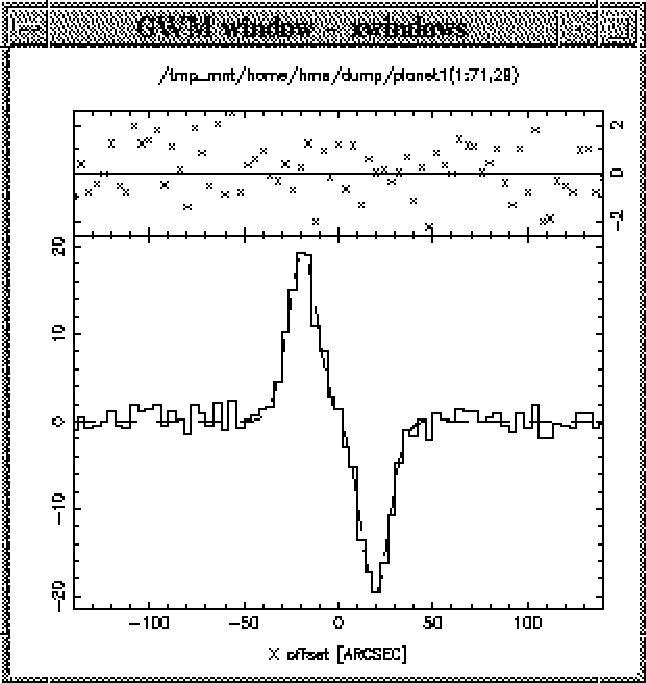
\includegraphics[height=80mm]{sc1_fitgauss}
\end{center}

   While the `official' chop throw is 40 arc seconds, the fit reveals that
   it actually was 38.5 arc seconds.
   You can check the number in the data file with
\texttt{\xref{hdstrace}{sun102}{}}
   and correct it with
\texttt{\xref{setobj}{sun86}{SETOBJ}}

\begin{terminalv}
% hdstrace rxa_146mcse.more.jcmt.map.chop_thrw

RXA_146MCS.MORE.JCMT.MAP.CHOP_THRW  <_REAL>

  CHOP_THRW      40

% setobj value=38.5 object=rxa_146mcse.more.jcmt.map.chop_thrw
\end{terminalv}



   The next stage is to create a
\htmlref{single-beam map.}{glossdualbeam}
   There are two ways of doing this: One is to use a
   maximum entropy technique
(see Section~\ref{dbmem}).
   Those who go that route will re-join us
   after the RA/Dec maps have been accomplished.

   The more normal method of proceeding
   is to carry out a two-stage process of first restoring to a single-beam map
   and then converting this to an RA/Dec grid. Users of
\htmlref{NOD2}{glossnod2}
   will be familiar with this process. The maps will be calibrated as an
   intermediate step while they are single-beam Az/El maps.


\subsection{\label{restore}\xlabel{restore}Single-beam restoration}

   Use the routine
\texttt{\xref{restore}{sun132}{RESTORE}}
   to restore to a single-beam map. This uses the algorithm first outlined by
\htmltex{\ref{reference}}Emerson, Klein \& Haslam (1979){}
   for dealing with dual-beam mapping data. The algorithm is exactly the
   same as that used in the NOD2 routine \texttt{restore}. To illustrate
   the result, we use
\texttt{\xref{display}{sun95}{DISPLAY}}
   and
\texttt{\xref{lutneg}{sun95}{LUTNEG}}.

\begin{terminalv}
% restore input=rxa_146mcse output=rxa_146mcser
Map was scanned along x-cells
ratio of beams = 1.000
separation of beams=  38.5 arcseconds
% display rxa_146mcser accept
% lutneg
\end{terminalv}

\begin{center}
\leavevmode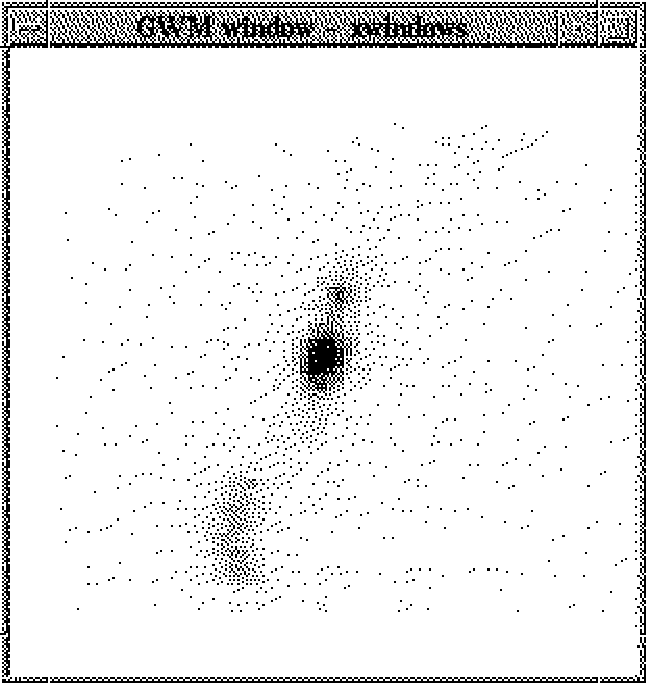
\includegraphics[height=80mm]{sc1_display4}
\end{center}

\subsection{\label{calib}\xlabel{calib}Calibration}

   If you went through the whole process so far for each map, you should
   now have a number of beam maps (usually planet maps) for calibration
   purposes and a number of source maps that you want to calibrate. All
   these are in single-beam Az/El format.

   There are two ways to get calibrated information out of the maps. One
   is to integrate the data as they are over regions of interest and to
   convert the pixel sum in mV into a
\htmlref{flux density}{glossflux}
   in Jy. The other is to calibrate the data by multiplying each pixel
   so that it gives the
\htmlref{intensity}{glossflux}
   in Jy/beam, MJy/sr, Jy/pixel etc.

   However, there are a few things to remember. Firstly, make sure you
   use the nearest
\htmlref{planet map}{glossplanetmap}
   in time and elevation to your source map. Next, if the planet map was
   made with a different
\htmlref{sensitivity setting}{glosssensset}
   from the source map, then this must be taken into account in your
   calculation. For instance, if the planet map was made with a
   sensitivity of 10 mV, and the source with 5 mV, then you must
   \textit{halve\/} the conversion factor obtained for the planet before
   converting the source into Jy. Also remember to take account of the
\htmlref{error beam}{glosserrorbeam}
   when measuring flux densities of extended
   sources which have been calibrated against beam maps made of point
   sources. Check with your support scientist if you are unsure of this.



   A simple way to evaluate the beam maps is to use
\texttt{\xref{stats}{sun95}{STATS}}
   on an area that is sure to contain all the signal from the
   calibration source. This returns both the `flux density' in mV and
   the peak intensity in mV. The peak intensity is just the brightest
   pixel in the area, it would be better to
   fit a Gaussian profile to the beam
(See Section~\ref{beam})
   and use the fitted peak intensity.

\begin{terminalv}
% stats planet2\(-20.:20.,-20.:20.\)

  Pixel statistics for the NDF structure
  /tmp_mnt/home/hme/dump/planet2(31:41,24:34)

     Title                     : KAPPA - Sub
     NDF array analysed        : DATA

        Pixel sum              : 445.3396
        Pixel mean             : 3.680492
        Standard deviation     : 5.134146
        Minimum pixel value    : -3.51409
           At pixel            : (31, 25)
           Co-ordinate         : (-20, -16)
        Maximum pixel value    : 21.22465
           At pixel            : (36, 29)
           Co-ordinate         : (0, 0)
        Total number of pixels : 121
        Number of pixels used  : 121 (100.0%)
\end{terminalv}

   The first conversion factor (to work out flux densities from pixel
   sums) follows from the comparison of the flux density of the
   calibration source and the pixel sum over its map. If the planet is
   known to have been 520 Jy, then

\[c_1 = 520\,{\rm Jy} / 445\,{\rm mV} = 1.17\,{\rm Jy/mV}\]

   The second conversion factor (to work out intensities from pixel
   values) follows from the comparison of the peak intensity of the
   calibration source and the peak pixel value. The expected peak
   intensity for a top-hat source of \textit{R\/} = 3 arc seconds radius
   (such as a planet) follows from its total flux density:

\[{I_{\nu,\rm max} \over {\rm Jy}/beam}
    = {S_{\nu} \over {\rm Jy}}
    \, {1 - \exp(-x^2) \over x^2}
\mbox{\ \ \ \ where\ \ }
  x = {R \over 0.6\,H\!P\!BW}\]

   where
\htmlref{HPBW}{glosshpbw}
   = 18 arc seconds in our example. The peak intensity then is 500
   Jy/beam and the second conversion factor

\[c_2 = {500\,{\rm Jy}/beam \over 21\,{\rm mV}}
      =  24\,{{\rm Jy}/beam \over     {\rm mV}}\]

   Although it is common to use the beam size as the unit of solid
   angle, this is confusing. We can express the beam size in steradian
   to find

\[c_2 =  24\,{{\rm Jy/mV} \over \pi (H\!P\!BW/2)^2}
      = 4010\,{\rm MJy/sr \over mV}\]

   To calibrate a map in Jansky per pixel, we would use the fact that
   the pixels measure 4 arc seconds squared. Hence there are 2660
   million pixels in a steradian.

\[c_2 = 4010\,{{\rm MJy/mV}   \over 2.66\,10^9\,pixel}
      =  1.5\,{{\rm Jy}/pixel \over {\rm mV}}\]

   All these conversion factors assume that the calibration map was
   taken with the same sensitivity setting as the source map. The
   correct conversion factor is proportional to the sensitivity
   setting. In our example, the planet might have been observed with a
   setting of 10 mV and the source with 5 mV. Hence we calibrate the
   source map in MJy/sr by multiplying it with 2005.
   Multiplication of data with a constant is achieved with
\texttt{\xref{cmult}{sun95}{CMULT}}
   and a units string can be set with
\texttt{\xref{setunits}{sun95}{SETUNITS}}:

\begin{terminalv}
% cmult rxa_146mcser 2005 rxa_146mcsern
% setunits rxa_146mcser MJy/sr
\end{terminalv}

\subsection{\label{ae2rd}\xlabel{ae2rd}Celestial coordinates}

   After the maps are calibrated use the routine
\texttt{\xref{ae2rd1}{sun132}{AE2RD1}}.
   This application will transform JCMT map data into a tangent plane
   image centred on a specified right ascension and declination. The
   re-binning is performed by convolving the input data with a truncated
   Bessel function. It is similar but not identical to the NOD2 function
   \texttt{convert}. Another option is to use the routine
\texttt{\xref{ae2rd2}{sun132}{AE2RD2}},
   which carries out the same process using the interpolation method of
\htmlref{Renka \& Cline (1984).}{refer}
   In either case it is possible to process up to ten
   Az/El input maps to make a single RA/Dec map, to weight the maps according
   to their relative signal-to-noise, and to introduce relative pointing
   corrections between the maps. The noise level of the map can be
   estimated using
\texttt{\xref{stats}{sun95}{STATS}}
   on a region of the map away from any
   sources. The centre position of the output map will default to the
   centre of the first input map, or alternatively can be entered
   manually. To illustrate
   the result, we use
\texttt{\xref{display}{sun95}{DISPLAY}}
   and
\texttt{\xref{lutneg}{sun95}{LUTNEG}}.

\begin{terminalv}
% ae2rd1 b1950=f output=omc1
Re-binning by Bessel function convolution.
INFILE - The name of a file containing JCMT map data /''/ > rxa_146mcsern
AE2RD1 - No pointing corrections applied
INFILE - The name of a file containing JCMT map data /'END'/ >
Coordinates are FK5 J2000.0
RA_CENTRE - The RA of the centre of the output map /'+05 35 14.37'/ >
DEC_CENTRE - The Dec. of the centre of the output map /'-005 22 32.3'/ >
% display omc1 badcol=red axes=t low=-2500 high=35000 accept
% lutneg
\end{terminalv}

\begin{center}
\leavevmode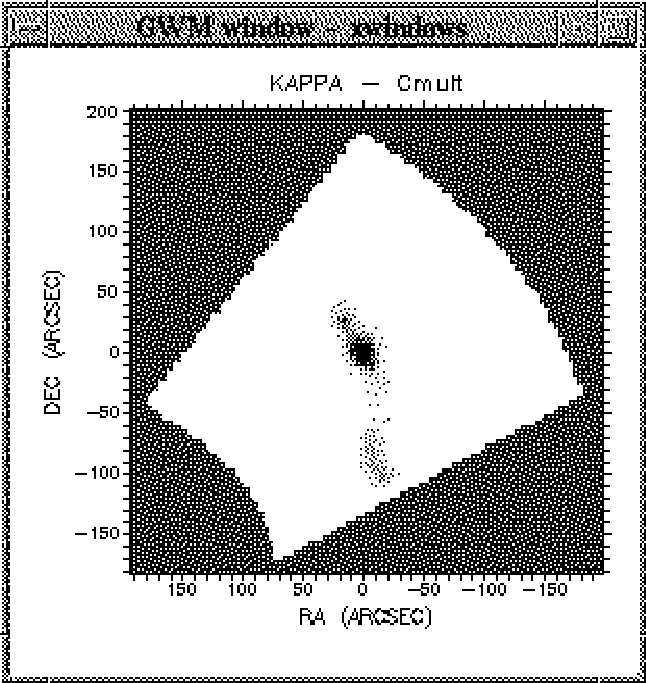
\includegraphics[height=80mm]{sc1_display5}
\end{center}

\newpage
\section{Analysis}

\subsection{\label{spindex}\xlabel{spindex}Spectral index map}

   As an example of further analysis, we show how two maps at different
   frequencies can be combined into a map of the spectral index

\[\alpha = {\lg(I_1/I_2) \over \lg(\nu_1/\nu_2)}\]

   We begin with two maps, say at 450 GHz and 225 GHz. The low-frequency
   map is sampled at twice the pixel step, so that both have the same
   number of pixels per beam
\htmlref{(HPBW}{glosshpbw}
   = 2.5 pixel in our case).

\begin{center}
\leavevmode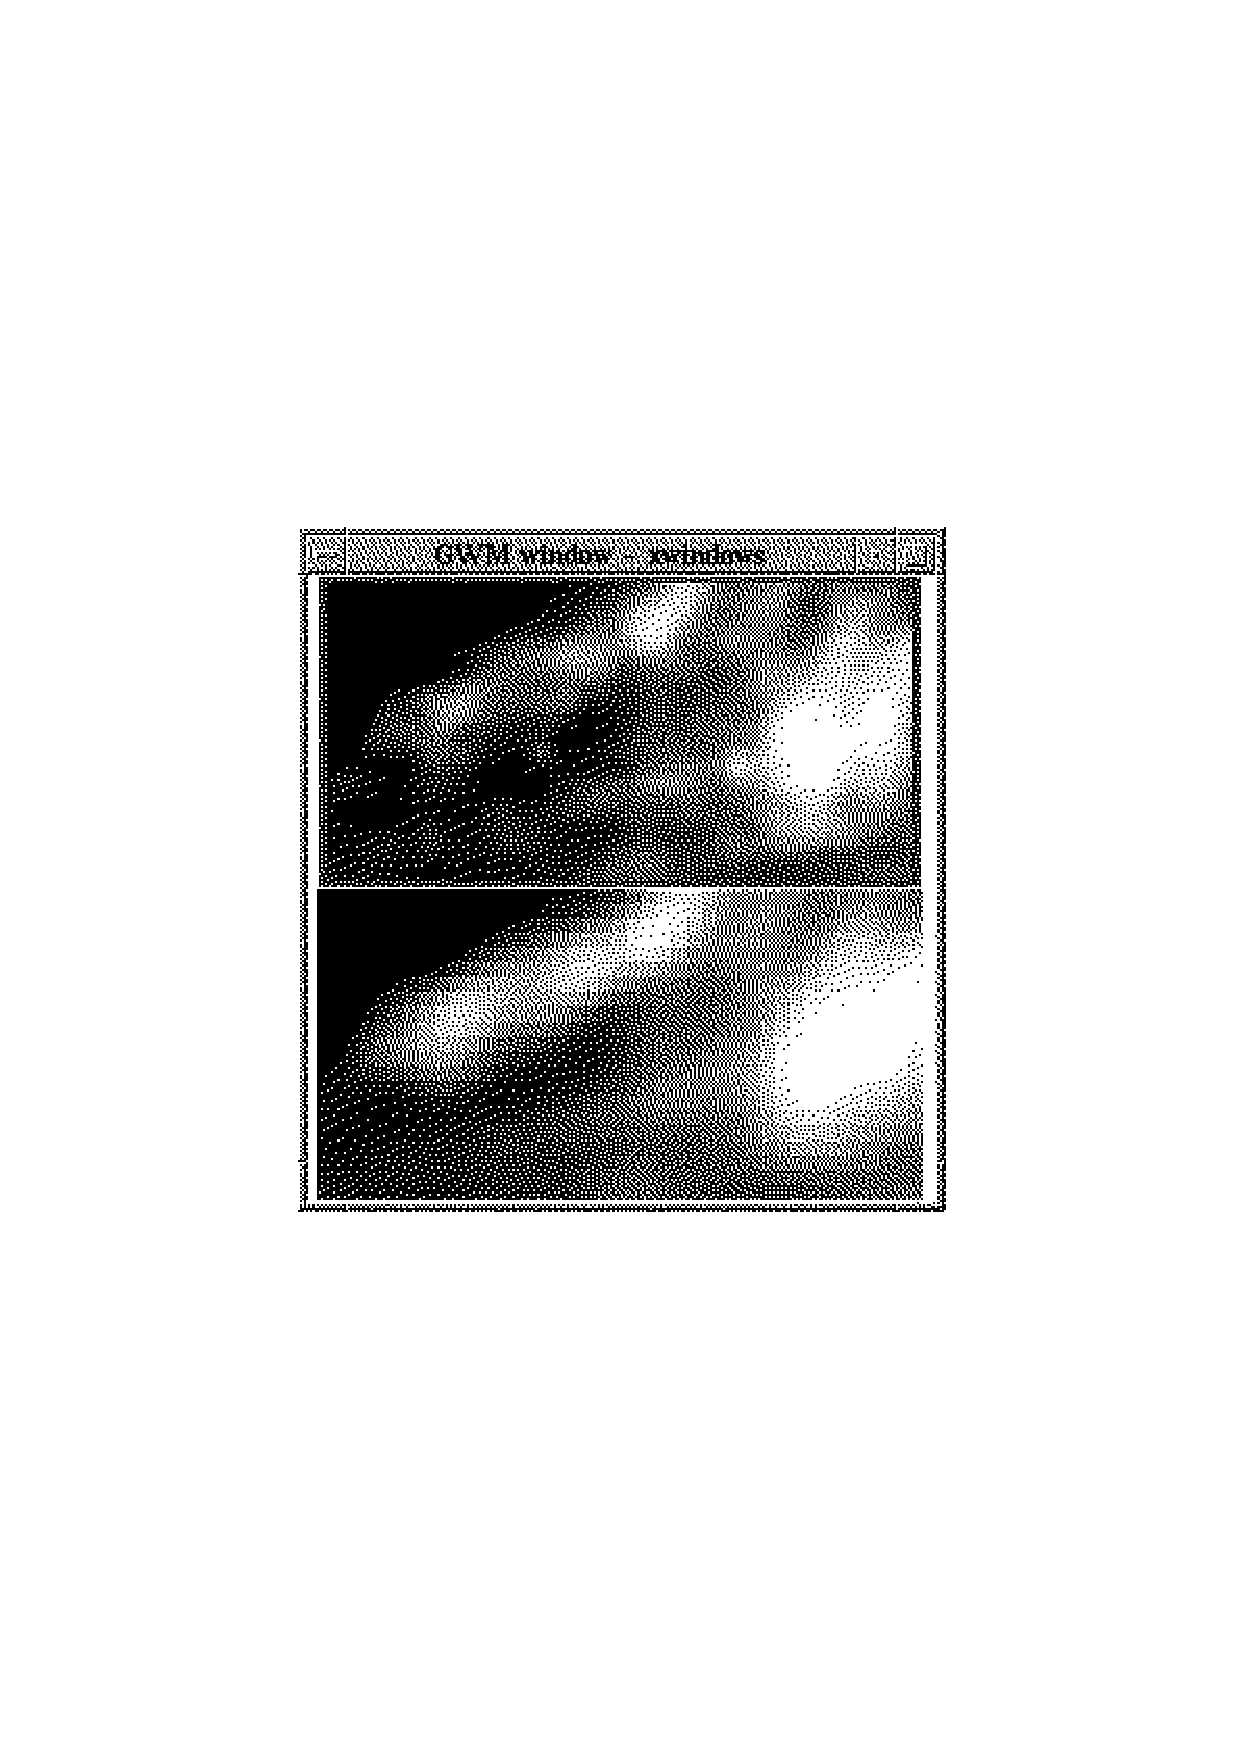
\includegraphics[height=80mm]{sc1_spindex1}
\end{center}

   Both maps cover the same area, i.e.\ the centres of their end pixels
   coincide, and so does the centre pixel.
   First we must smooth the high-frequency map to the resolution of the
   low-frequency map. To smooth from 2.5 pixel to 5 pixel HPBW we
   use a Gaussian smoothing function (the application
\texttt{\xref{gauss}{sun95}{GAUSMOOTH}})
   with 4.33 pixel HPBW.

\begin{terminalv}
% gauss in=freqhi fwhm=4.33 out=freqhi_s
\end{terminalv}

   \textit{Note that we use a
\xref{KAPPA}{sun95}{}
   routine here.
\xref{Figaro}{sun86}{}
   has a routine of the same name, but for a completely different
   purpose. Depending on the order of your
\htmlref{package activations,}{start}
   you may get the wrong application here.
   The next version of KAPPA (0.9) will rename the Gauss smoothing
   command to\/ \tt gausmooth}.

   Now we have to pick only each second pixel from the high-frequency
   map to get the same sampling as the low-frequency map. Unfortunately,
   the KAPPA routines for re-sampling are obsessed with pixels, and also
   a bit stupid. Here we use
\texttt{\xref{compick}{sun95}{COMPICK}},
   which picks only
   the 1st, 3rd, 5th, etc.\ pixels from the input. Our maps have an
   odd number of pixels, so that they have a central pixel. As they are,
   \texttt{compick} would not take the last pixel, even though it is an
   odd pixel. This is because the even pixel belonging to it is
   not there. (Such procedure makes sense in the sister application
\texttt{\xref{compave}{sun95}{COMPAVE}}
   that would average each odd pixel with the ones to
   its right, top, and top-right.)
   Therefore, before \texttt{compick} we
   will make the map one pixel larger on the right and at the top by
   using
\texttt{\xref{ndfcopy}{sun95}{NDFCOPY}}
   on a superset of the map (which is technically an
\htmlref{NDF section).}{glossndfsection}

   After \texttt{compick} the axis data have disappeared. Due to our
   careful preparations, the pixel centre coordinates should have the
   same range as in the original, or the same as in the low-frequency
   map. You can copy the axis from the low-frequency map with
\texttt{\xref{copobj}{sun86}{COPOBJ}}.

\begin{terminalv}
% ndfcopy freqhi_s\(:82,:42\) temp
% compick temp compress=2 outpick=freqhi_sr
Array is 82 by 42 pixels
x dimension of output array  =  41
y dimension of output array  =  21
% rm temp.sdf
% copobj freqlo.axis freqhi_sr.axis
\end{terminalv}

   You can imagine that things get really tricky when the sampling rates
   differ not by an integer factor. You would rely on
\texttt{\xref{sqorst}{sun95}{SQORST}}
   to `squash or stretch' a map to a new number of pixels.

   \textit{The next version of KAPPA (0.9) will have a new command\/
\texttt{\xref{transformer}{sun239}{TRANSFORMER}},
   which may be better suited to the task of re-sampling.}

   The actual calculation of the spectral index map is now trivial,
   thanks to the application
\texttt{\xref{maths}{sun95}{MATHS}},
   which can combine up to 26 images and 26 numeric parameters using a
   user-specified mathematical expression.

\begin{terminalv}
% maths
EXP - Expression /''/ > (log10(ia)-log10(ib))/(log10(450)-log10(225))
IA - Input NDF structure > freqhi_sr
IB - Input NDF structure > freqlo
OUT - Output NDF structure > spindex
\end{terminalv}

\begin{center}
\leavevmode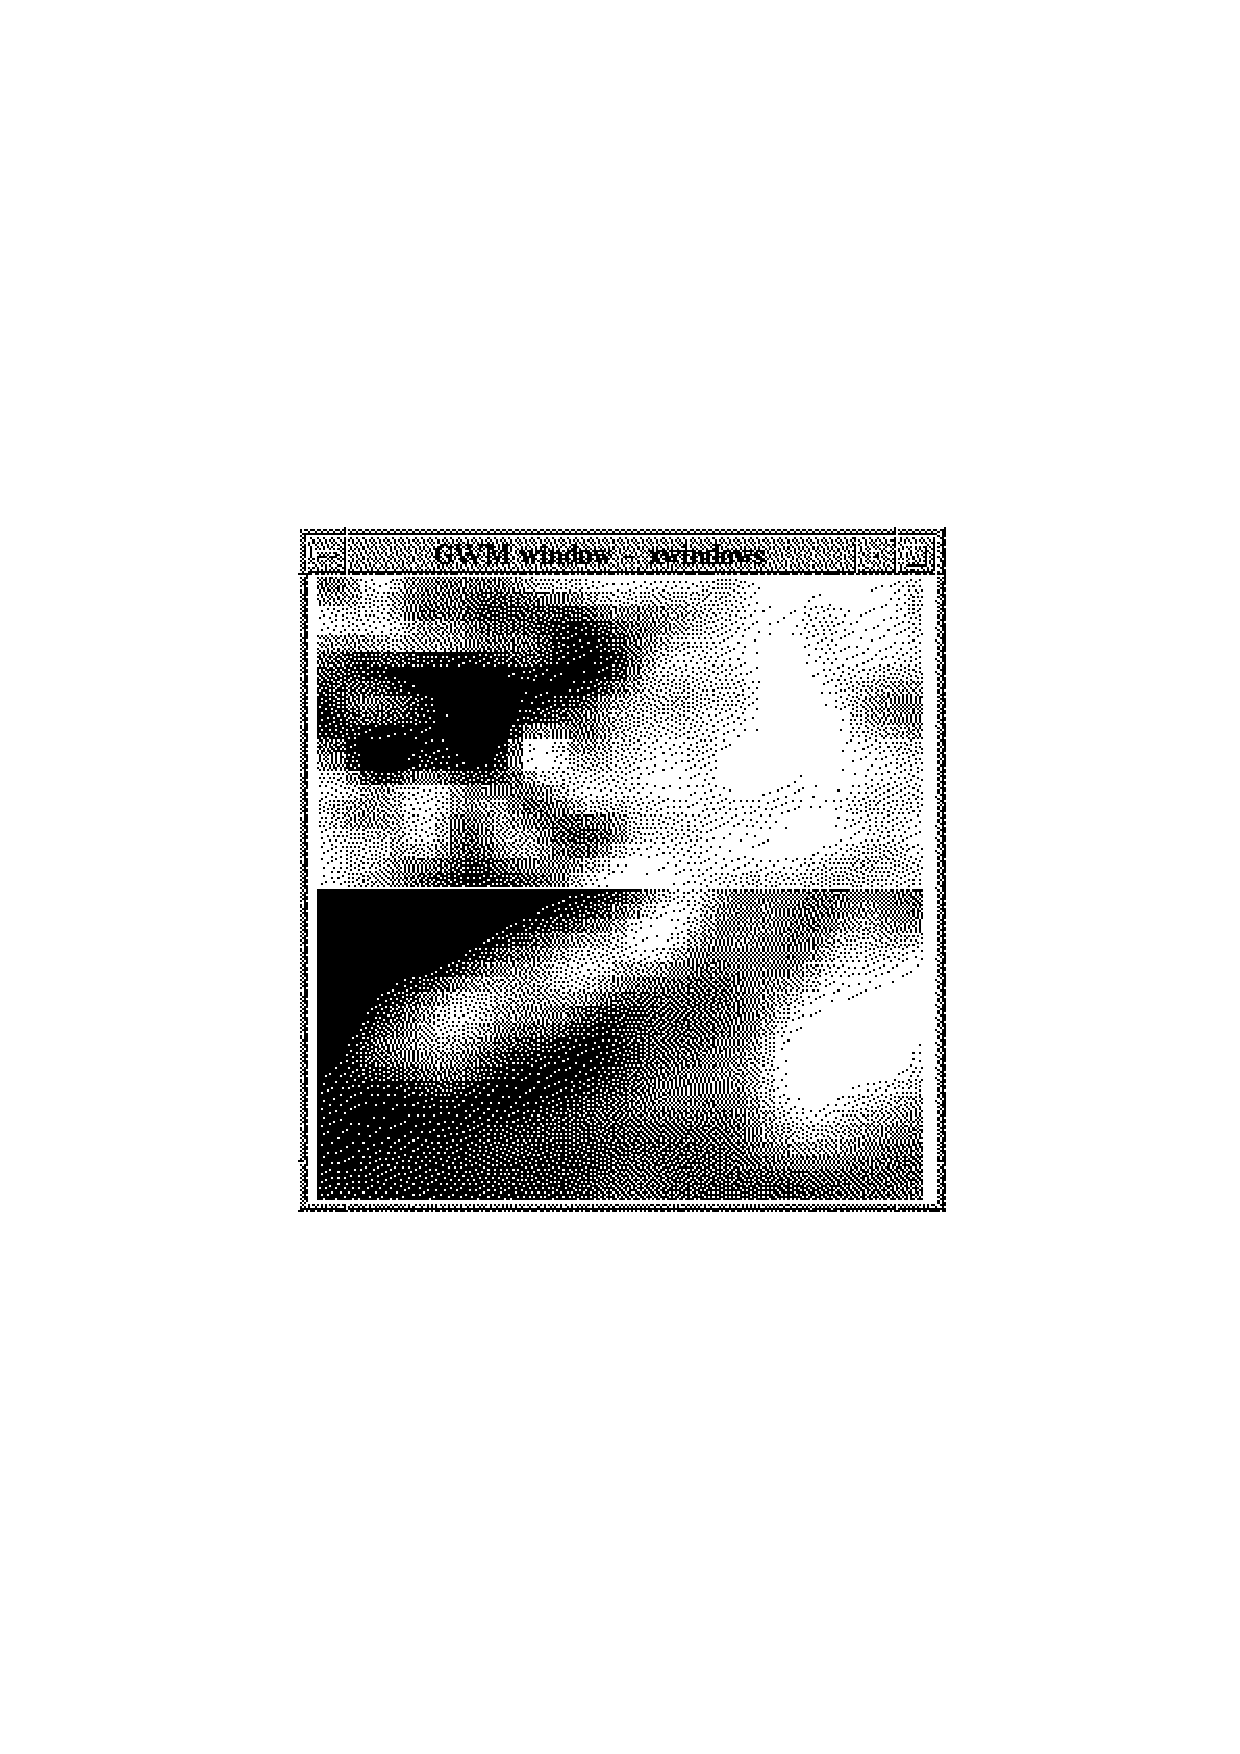
\includegraphics[height=80mm]{sc1_spindex2}
\end{center}

   The JCMT extension to the data
   will be wrong after the re-binning operations. As with the axis data,
   the JCMT extension of the low-frequency map are largely valid
   for the spectral index map. (The things used during the reduction,
   like local sidereal time, are not valid, but anything to do with
   celestial coordinates should be fine.) Hence you might remove the
   existing extension with
\texttt{\xref{erase}{sun95}{ERASE}}
   and then copy like this:

\begin{terminalv}
% erase spindex.more.jcmt
% copobj freqlo.more.jcmt spindex.more.jcmt
\end{terminalv}

\subsection{\label{iras90}\xlabel{iras90}Exporting to IRAS90}

\xref{IRAS90}{sun163}{}
   is an application package written specifically to work with IRAS
   data. However, the
\htmlref{tangent-plane projection we got for our JCMT map}{ae2rd}
   is quite suitable for use
   with IRAS90 applications. This is especially true if the maps were
\htmlref{calibrated in MJy/sr}{calib}
   or some other unit understood by IRAS90.

   In order to use maps in IRAS90, they must have at least part
   of the data format extension specific to IRAS90. For JCMT maps you
   can add the astrometry information with the command
\texttt{\xref{iras\_tag}{sun132}{IRAS_TAG}}.
   (Note that the relevant parts of the JCMT extension must be correct
   for this to work. Namely, you must not re-bin the map between
\texttt{\xref{ae2rd1}{sun132}{AE2RD1}}
   and \texttt{iras\_tag}.) You also have to generate the image information
   `by hand', using some basic HDS manipulators
(\texttt{\xref{creobj}{sun86}{CREOBJ}}
   and
\texttt{\xref{setobj}{sun86}{SETOBJ}})
   from
\xref{Figaro.}{sun86}{}
   In doing so, we tell deliberate lies to IRAS90, to overcome its
   specialisation on IRAS data. Finally we have a look at the result with
\texttt{\xref{hdstrace}{sun102}{}}.

\begin{terminalv}
% iras_tag input=omc1
% creobj type=IMAGE_INFO dims=0 object=omc1.more.iras.image_info
% creobj type=_CHAR\*6 dims=0 object=omc1.more.iras.image_info.instrument
% setobj value=SURVEY object=omc1.more.iras.image_info.instrument
% creobj type=_INTEGER dims=0 object=omc1.more.iras.image_info.band
% setobj value=1 object=omc1.more.iras.image_info.band
% creobj type=_CHAR\*8 dims=0 object=omc1.more.iras.image_info.type
% setobj value=UNKNOWN object=omc1.more.iras.image_info.type
% hdstrace omc1.more.iras

STRUCT.MORE.IRAS  <IRAS_EXTENSION>

  ASTROMETRY     <IRAS_ASTROMETRY>   {structure}
     STATE          <_CHAR*10>      'DEFINED'
     PROJ_NAME      <_CHAR*15>      'GNOMONIC'
     SCS            <_CHAR*25>      'EQUATORIAL(B2000)'
     EPOCH          <_DOUBLE>       2000
     PROJ_PARS(8)   <_DOUBLE>       1.46275826443488,-0.09382259800936,
                                    ... 0.00001939254724,0,0

  IMAGE_INFO     <IMAGE_INFO>    {structure}
     INSTRUMENT     <_CHAR*6>       'SURVEY'
     BAND           <_INTEGER>      1
     TYPE           <_CHAR*8>       'UNKNOWN'

End of Trace.
\end{terminalv}


\subsection{\label{grid}\xlabel{grid}Hardcopy with coordinate grid}

   The recommended way to get coordinate overlays and/or text on top of
   a map display (grey, colour, or contour), is to use
\texttt{\xref{skygrid}{sun163}{SKYGRID}}
   and
\texttt{\xref{skywrite}{sun163}{SKYWRITE}}
   from the
\xref{IRAS90}{sun163}{}
   package.

   In order to use maps in IRAS90, they must have at least part
   of the data format extension specific to IRAS90. See
Section~\ref{iras90}.

   Here we set ourselves the task to produce a colour hardcopy of our
   map with a coordinate overlay. Instead of the graphics device `xw' we
   have to use `epsfcol\_p'. Each application that contributes to the
   plot, will write one Encapsulated PostScript file. In the end we
   combine them all into a single PostScript file that we can print. If
   you prefer grey PostScript, use the device `epsf\_p'. If you rather
   use a landscape orientation of the paper, use `*\_l' instead of `*\_p'.

   In order that the printout is what you expect, you should perhaps try
   everything first on the `xw' device. The only difference in the
   command parameters is the magnification in
\texttt{\xref{display}{sun95}{DISPLAY}},
   because
   the PostScript device has smaller pixels and therefore needs higher
   magnification. Use the default offered as a guideline, since it is
   always the highest magnification possible without cutting off the
   edges of the image.

   We begin by removing any old PostScript files that might confuse us
   later. All PostScript output from Starlink software goes into files
   with names \texttt{gks74.ps}), \texttt{gks74.ps.1}, \texttt{gks74.ps.2},
   etc. It's easy to pick the wrong one with these names.

\begin{terminalv}
% rm gks74.ps*
\end{terminalv}

   Next we use \texttt{display}. We do not clear the display, since that
   would only create an extra PostScript file without any graphics in
   it. We also specify the colour lookup table to \texttt{display},
   since this is the only way to do it: We cannot use a dedicated
   command for reading a lookup table, since it would affect only the
   PostScript file it creates,
   not the one that \texttt{display} creates. Since we print on white
   paper and have many bad values in our map, we ask to plot those in
   white. We do not want the axes from \texttt{display}, but we want
   some space left for annotation. Therefore, we reduce the
   magnification to 2/3 or 3/4 the default.

\begin{terminalv}
% display prompt
SCALE - Scale the data? /YES/ >
COMP - Component to display /'Data'/ >
IN - NDF to be displayed /@omc1/ >
COSYS - Co-ordinate system /'Data'/ >
CLEAR - Is the current picture to be cleared before display? /FALSE/ >
DEVICE - Name of display device /@xw/ > epsfcol_p
LUT - NDF containing lookup table /!/ > /home/hme/luts/paslin_lut(,2:)
NN - Nearest-neighbour mapping of lookup table? /NO/ >
MODE - Method to define the scaling limits /'SCALE'/ >
AXES - Are annotated axes to be drawn? /NO/ >
BORDER - Is a coloured border required? /NO/ >
BADCOL - Colour of bad pixels /'white'/ >
FILL - Fill the plotting area? /NO/ >
CENTRE - Position at the centre of the display /[-2,10]/ >
XMAGN - Magnif. in X co-ordinate about the centre of array /23.08158/ > 15
YMAGN - Magnif. in Y co-ordinate about the centre of array /15/ >
LOW - Low value for display /-71414.210937/ > -2500
HIGH - High value for display /45424.492188/ > 35000
SCALOW - Object to contain the lower scaling value. /0/ >
SCAHIGH - Object to contain the upper scaling value. /0/ >
OUT - NDF for scaled data /!/ >
\end{terminalv}

   Now we run \texttt{skygrid} to get an RA/Dec grid. We specify
   `equatorial' and will get B1950. Since the map is in J2000, the lines
   will be shifted and rotated a bit. Then we run \texttt{skygrid} a
   second time to get some galactic coordinates without annotation.

\begin{terminalv}
% skygrid prompt
MSG_FILTER - Level of information to be displayed /'NORMAL'/ >
DEVICE - Name of display device /@xw/ > epsfcol_p
CLEAR - Clear the graphics window? /NO/ >

 DATA picture "KAPPA_DISPLAY" being used
 The picture covers the image section ( 1:98, 1:96 )
IN - The displayed NDF /@omc1/ >

COORDS - Sky coordinate system /'EQUATORIAL'/ >
LABEL - Annotate the coordinate grid? /YES/ >
TEXTSIZE - Size of annotation text. /0.02/ >
COORDSIZE - Size of text used for formatted coordinate values. /0.01/ >
TOLERANCE - Tolerance for the plotting of the grid lines /6/ > 0
LINES - Grid lines across the image? /NO/ > y
LONINT - Right Ascension (B1950) interval between grid marks /'0'/ >
LATINT - Declination (B1950) interval between grid marks /'0'/ >
LONACC - Right Ascension (B1950) accuracy /'0'/ >
LATACC - Declination (B1950) accuracy /'0'/ >
PENA - Pen number used to draw boundary /3/ > 1
PENB - Pen number used to draw curves and tick marks /3/ > 1
PENC - Pen number used to draw text labels /1/ >
PEND - Pen number used to draw coordinate labels /1/ >

% skygrid prompt
MSG_FILTER - Level of information to be displayed /'NORMAL'/ >
DEVICE - Name of display device /@xw/ > epsfcol_p
CLEAR - Clear the graphics window? /NO/ >

 DATA picture "KAPPA_DISPLAY" being used
 The picture covers the image section ( 1:98, 1:96 )
IN - The displayed NDF /@omc1/ >

COORDS - Sky coordinate system /'EQUATORIAL'/ > GALACTIC
LABEL - Annotate the coordinate grid? /YES/ > no
TOLERANCE - Tolerance for the plotting of the grid lines /6/ > 0
LINES - Grid lines across the image? /NO/ > y
LONINT - Galactic Longitude interval between grid marks /'0'/ > .05
LATINT - Galactic Latitude interval between grid marks /'0'/ > .05
LONACC - Galactic Longitude accuracy /'0'/ >
LATACC - Galactic Latitude accuracy /'0'/ >
PENA - Pen number used to draw boundary /1/ >
PENB - Pen number used to draw curves and tick marks /1/ >
PENC - Pen number used to draw text labels /1/ >
PEND - Pen number used to draw coordinate labels /1/ >
\end{terminalv}

   Now we use \texttt{skywrite} with B1950 coordinates to indicate what
   galactic meridians and parallels have been drawn.

\begin{terminalv}
% skywrite attribute=pen mode=keyboard coords=equa
DEVICE - Name of display device /@xw/ > epsfcol_p

 DATA picture "KAPPA_DISPLAY" being used
 Using astrometry information stored with the picture in the
 AGI database
PEN - Pen number used to write text /1/ >
ATTRIBUTE - Text attribute to set /'DEFAULT'/ > show

 DIRECTION: text up direction - ( 0, 0 )
 HEIGHT: text height as a fraction of X size of the image - 0
 ASPECT_RATIO: character aspect ratio (width/height) - 0
 JUSTIFICATION: text justification -
 SPACE: space between characters - 0
 FONT - GKS font number - 0
 PEN - pen number - 1

ATTRIBUTE - Text attribute to set /'DEFAULT'/ > dir
DIRECTION - Text up-vector /[0,1]/ >
ATTRIBUTE - Text attribute to set /'DEFAULT'/ > hei
HEIGHT - Text height /0.02/ > .01
ATTRIBUTE - Text attribute to set /'DEFAULT'/ > aspe
RATIO - Character aspect ratio (width/height) /0.66667/ >
ATTRIBUTE - Text attribute to set /'DEFAULT'/ > just
JUST - Text justification /'BL'/ >
ATTRIBUTE - Text attribute to set /'DEFAULT'/ > spac
SPACE - Space between characters /0/ >
ATTRIBUTE - Text attribute to set /'DEFAULT'/ > font
FONT - GKS font number /1/ >
ATTRIBUTE - Text attribute to set /'DEFAULT'/ > !
LON - Right Ascension (B1950) of the position /'209d'/ > 5h 32m 34s
LAT - Declination (B1950) of the position /'-19.45'/ > -5d 26m 30s
TEXT - Text to be written > '  209'
LON - Right Ascension (B1950) of the position /'5h 32m 34s'/ >
LAT - Declination (B1950) of the position /'-5d 26m 30s'/ > -5d 23m 30s
TEXT - Text to be written > '  208.95'
LON - Right Ascension (B1950) of the position /'5h 32m 34s'/ > 5h 32m 36s
LAT - Declination (B1950) of the position /'-5d 23m 30s'/ > -5d 21m
TEXT - Text to be written > -19.4
LON - Right Ascension (B1950) of the position /'5h 32m 36s'/ > 5h 32m 50s
LAT - Declination (B1950) of the position /'-5d 20m'/ > -5d 21m
TEXT - Text to be written > -19.35
LON - Right Ascension (B1950) of the position /'5h 32m 50s'/ > !
\end{terminalv}

   This leaves us with four Encapsulated PostScript files. We use the
\texttt{\xref{psmerge}{sun164}{}}
   utility in its simplest form to combine the four
   component plots into one:

\begin{terminalv}
% psmerge gks74.ps* > figure.ps
% rm gks74.ps*
\end{terminalv}

\begin{center}
\leavevmode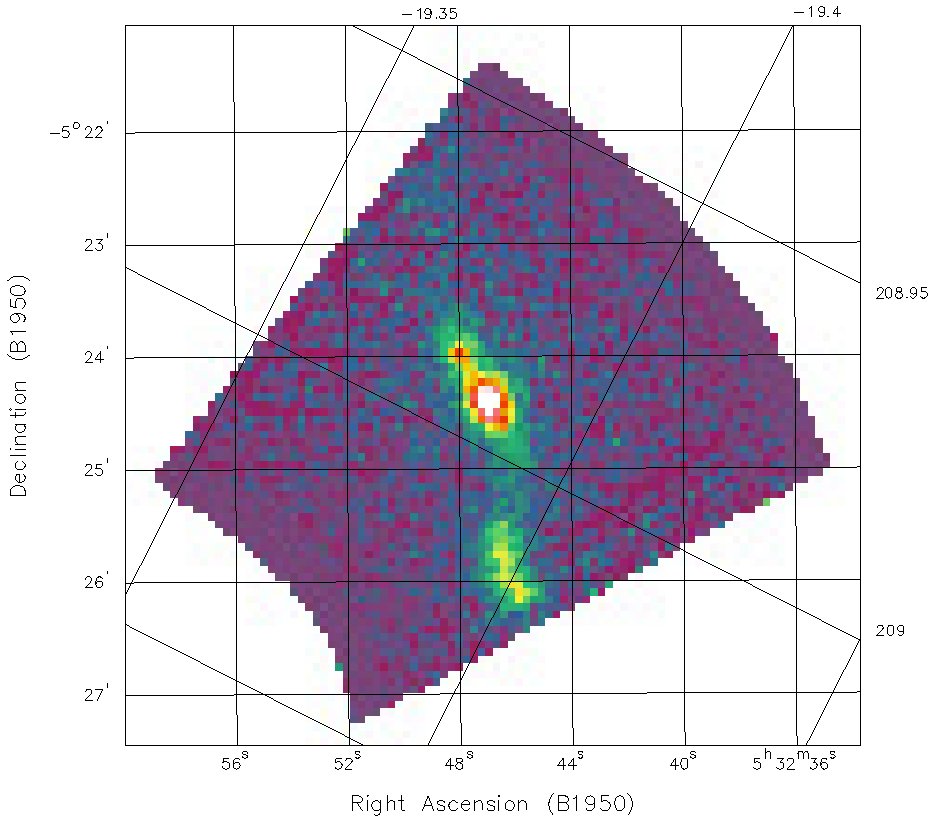
\includegraphics[height=100mm]{sc1_figure}
\end{center}

\subsection{\label{photo}\xlabel{photo}Photometry}

   The final process which users will typically wish to carry out on
   their data is to measure flux densities from point sources, or from
   extended regions of a map. There are many ways of doing this. For
   measuring extended rectangular regions the simplest way is to use
\texttt{\xref{stats}{sun95}{STATS}}.
   For complex regions a user can utilise the routines of
\xref{DAOPHOT,}{sun42}{}
   or the Starlink package
\xref{STARMAN.}{sun141}{}
   Alternatively, you can write the data in
\htmlref{FITS format}{glossfits}
   using the Figaro routine
\texttt{\xref{wdfits}{sun86}{WDFITS}},
   and use your favourite plotting package to make maps and obtain
   photometry. It is purely a matter of individual preference. However,
   the recommended route is to use the Starlink package
\xref{IRAS90.}{sun163}{}

   In order to use maps in IRAS90, they must have at least part
   of the data format extension specific to IRAS90. See
Section~\ref{iras90}.

   Once that is done, display the image in grey, colour, or as contour
   map and then run \texttt{skyphot}. Here we use
\texttt{\xref{display}{sun95}{DISPLAY}}
   and
\texttt{\xref{lutgrey}{sun95}{LUTGREY}}.

\begin{terminalv}
% display omc1 badcol=red clear=t low=-2500 high=35000 accept
% lutgrey
% skyphot prompt
MSG_FILTER - Level of information to be displayed /'NORMAL'/ >
IN - The input NDF /@omc1/ >
MODE - Source of input coordinates /'CURSOR'/ >
PLOT - Are graphics to be produced? /YES/ >
PEN - SGS pen number for graphics /3/ > 4
LOOP - Are multiple operations to be performed? /NO/ >
COORDS - Sky coordinate system /'GALACTIC'/ >
SHAPE - Aperture shape /'ELLIPSE'/ >
SINGLE - Should the application exit after a single position? /NO/ >
SIZE - Aperture size in arc-minutes /1/ > 0.5,1
BACKVAL - Background surface brightness in MJy/sr /0/ >
LOGFILE - A log file for storing displayed information /!/ >
 Displaying GALACTIC sky coordinates.

DEVICE - Name of display device /@xw/ >
 DATA picture "KAPPA_DISPLAY" being used

 Position the cursor at each aperture centre and press any button
 (position the cursor outside the image to exit).


   Centre                 : 208.993491, -19.384913
   Total flux density     : 557.0360 Jy
   Mean surface brightness: 14242.31 MJy/sr
   Standard deviation     : 10223.52 MJy/sr
   Used pixels in aperture: 104

   Centre                 : 209.015332, -19.399040
   Total flux density     : 316.0943 Jy
   Mean surface brightness: 8160.360 MJy/sr
   Standard deviation     : 4017.797 MJy/sr
   Used pixels in aperture: 103

   Centre                 : 208.987172, -19.374126
   Total flux density     : 207.2716 Jy
   Mean surface brightness: 5299.525 MJy/sr
   Standard deviation     : 5075.885 MJy/sr
   Used pixels in aperture: 104



MEAN - A dummy value to be replaced by the value of parameter MEAN /0/ >
FLUX - A dummy value to be replaced by the value of parameter FLUX /0/ >
SIGMA - A dummy value to be replaced by the value of parameter SIGMA /0/ >
\end{terminalv}

\begin{center}
\leavevmode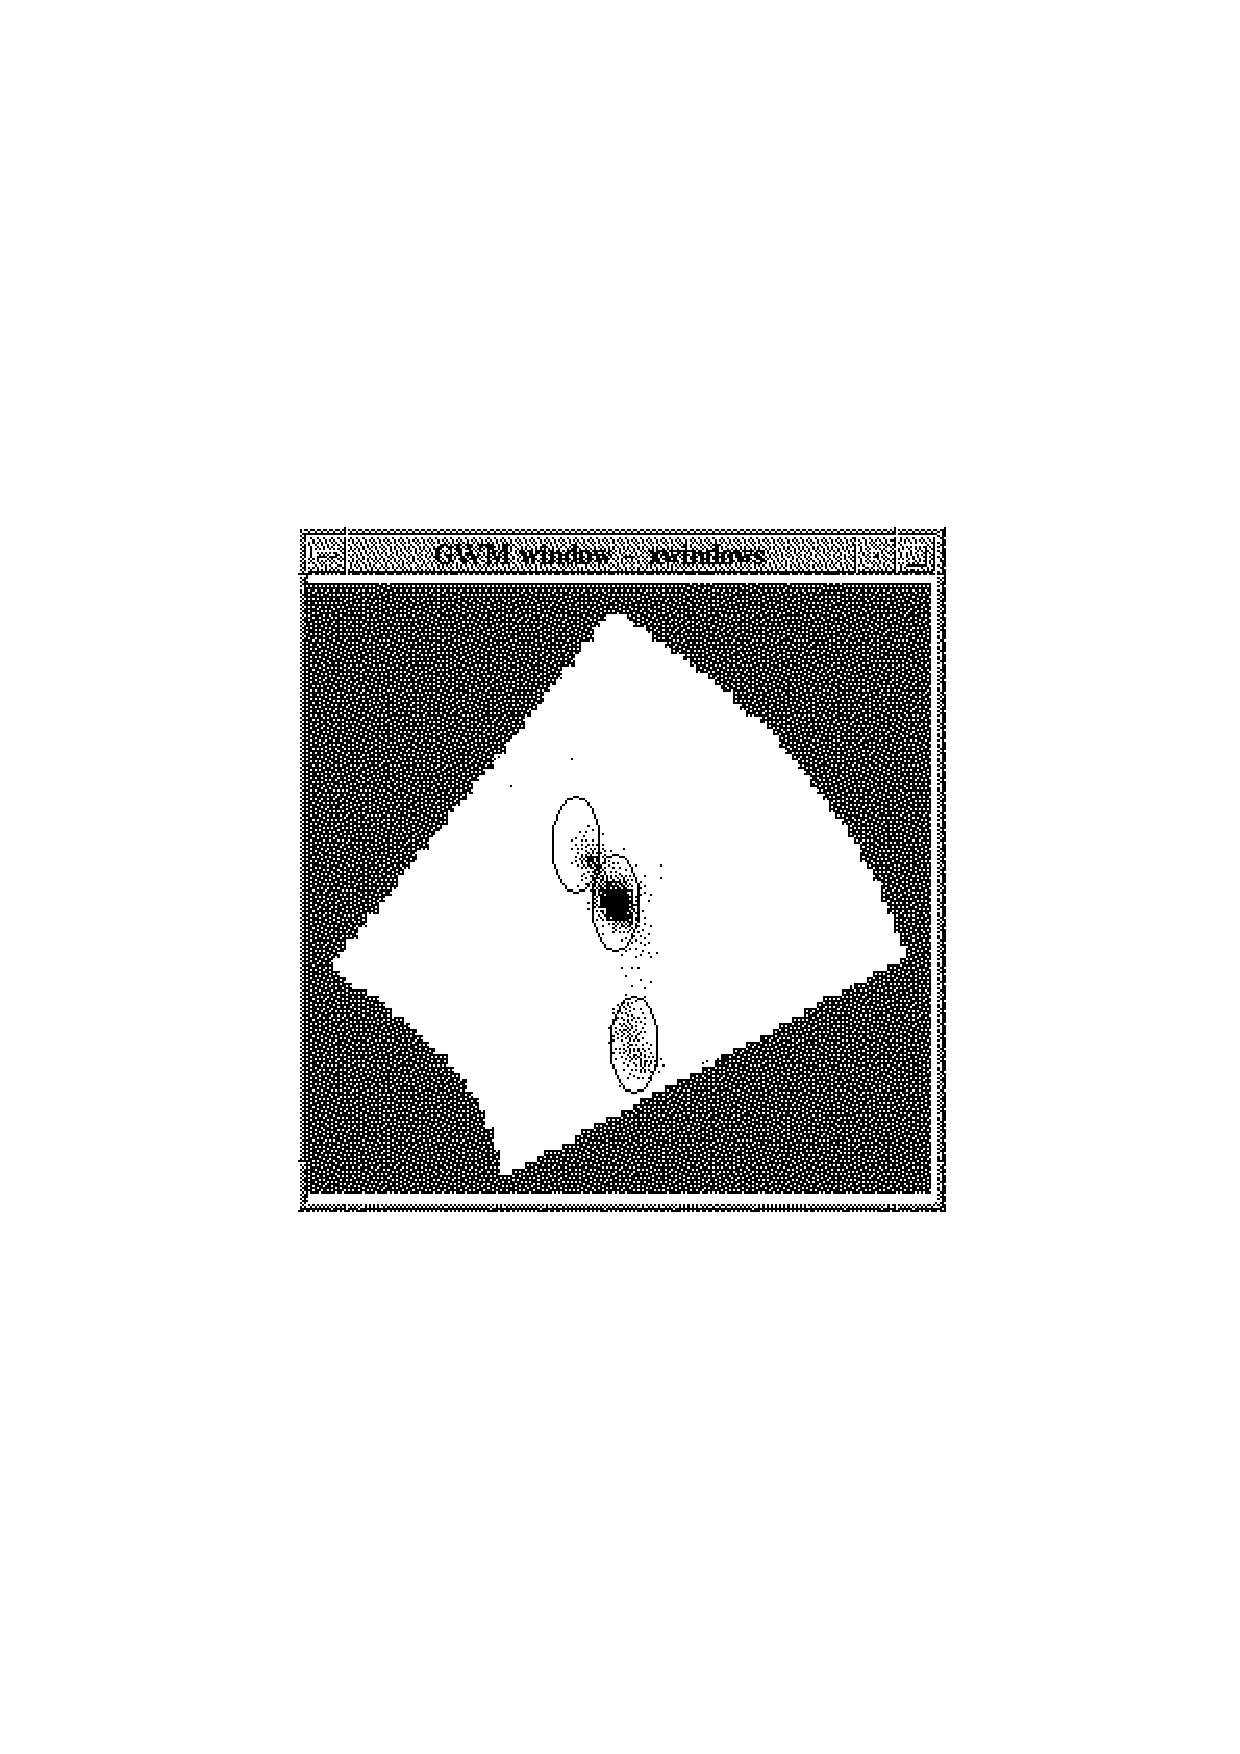
\includegraphics[height=80mm]{sc1_skyphot}
\end{center}

   Ellipses are not the only option for the photometric aperture. You
   can use rectangles or any polygon.


\newpage
\section{Further details on reduction}

\subsection{\label{start2}\xlabel{start2}Startup and on-line help}

   While some commands we use in this cookbook are utilities that are
   available without special action by the user, the application packages
   must each be activated. These are the commands to activate the
   packages
\xref{Figaro,}{sun86}{}
\xref{Specdre,}{sun140}{}
\xref{IRAS90,}{sun163}{}
\xref{KAPPA,}{sun95}{}
\xref{JCMTDR,}{sun132}{}
 and their responses:

\begin{terminalv}
% figaro

----------- Initialising for  Figaro ------------
             General data reduction
        Version 3.2-3  15 September 1994

         Type "fighelp figaro" for help
   or "fighelp news" for news on 3.1-1, 3.2, 3.2-3

%specdre

------------ Initialised for Specdre ------------
           Spectroscopy data reduction
            Version 1.0   17 Sep 1993

         Type "spe_help specdre" for help

% iras90

  IRAS90 commands are now available -- (Version 1.1)

  Type i90help for help on IRAS90 commands

% kappa

--     Initialised for KAPPA      --
--   Version 0.8-6U, 1994 June    --

   Type kaphelp for KAPPA help

% jcmtdr

------------ Initialised for JCMTDR ------------
          Version 1.2  10 January 1995

        Type "jcmt_help jcmtdr" for help
     or "jcmt_xhelp" to start the Web browser
\end{terminalv}

   All application packages provide on-line help via a command that is
   part of the package. When you activate each package
   it responds with a message that identifies the software version and
   also tells you what the help command for that package is.

   For example, JCMTDR offers on-line help via the command
\texttt{\xref{jcmt\_help}{sun132}{JCMT_HELP}}
   and it also has a command
\texttt{\xref{jcmt\_xhelp}{sun132}{JCMT_XHELP}}
   to start the
\xref{Mosaic}{sun175}{}
\htmladdnormallink{World Wide Web}{http://www.w3.org/hypertext/WWW/TheProject.html}
   browser for you with the
\xref{documentation on JCMTDR.}{sun132}{}

   If you are more of the `just let's try and run it' type, a good trick
   is to use the \texttt{prompt} keyword on the command. In that case
   the command will prompt you for every parameter it knows about. There
   are often hidden parameters that prevent you from discovering the
   most advanced features of a command.

   Whenever a command prompts you for the value of a parameter, and you
   don't know what it's on about, you can respond with a question mark.
   That should give you the on-line help for the parameter in question
   and then prompt you again. JCMTDR, unfortunately, gives only a
   useless minimum help in these circumstances.

\begin{terminalv}
% stats prompt
NDF - Data structure to analyse /@rxa_146m/ >
COMP - NDF array component to analyse /'DATA'/ >
CLIP - Clipping levels /!/ > ?

STATS

 Parameters

   CLIP

     CLIP( ) = _REAL (Read)
        An optional 1-dimensional array of clipping levels to be
        applied, expressed as standard deviations.  If a null value is
        supplied for this parameter (the default), then no iterative
        clipping will take place and the statistics computed will
        include all the valid NDF pixels.

        If an array of clipping levels is given, then the routine will
        first compute statistics using all the available pixels. It
        will then reject all those pixels whose values lie outside K
        standard deviations of the mean (where K is the first value
        supplied) and will then re-evaluate the statistics. This
        rejection iteration is repeated in turn for each value in the
        CLIP array.  A maximum of 5 values may be supplied, all of
        which must be positive. [!]

CLIP - Clipping levels /!/ >
LOGFILE - File for logging results /!/ >

  Pixel statistics for the NDF structure
  /tmp_mnt/home/hme/dump/rxa_146m

     Title                     : OMC1
     NDF array analysed        : DATA

        Pixel sum              : 21094.68
        Pixel mean             : 5.212425
        Standard deviation     : 0.464714
        Minimum pixel value    : 1.335313
           At pixel            : (41, 29)
           Co-ordinate         : (20, 0)
        Maximum pixel value    : 9.292433
           At pixel            : (31, 29)
           Co-ordinate         : (-20, 0)
        Total number of pixels : 4047
        Number of pixels used  : 4047 (100.0%)

MAXIMUM /0/ >
MEAN /0/ >
MINIMUM /0/ >
SIGMA /0/ >
TOTAL /0/ >
NUMBAD /0/ >
NUMGOOD /0/ >
NUMPIX /0/ >
\end{terminalv}

   Some of the parameters are output rather than input. You should just accept
   the default values for those.

\subsection{\label{trace1}\xlabel{trace1}GSD file inspection}

   You can inspect a GSD file with
\texttt{\xref{gsd\_print}{sun132}{GSD_PRINT}},
   but be aware that the output is extremely long: It contains all the
   image data and whatever else came from the telescope, converted into
   a printable format.

\begin{terminalv}
% gsd_print rxa_146.dat
-----------------------------------------------------------------
 G S D     P R I N T
-----------------------------------------------------------------

 FILENAME     : rxa_146.dat
 GSD VERSION  :  4.000
 LABEL        : JCMT
 NITEMS       : 131


 NAME            UNIT          TYPE      TABLE     VALUE or SIZE
-----------------------------------------------------------------

 C1TEL                         C         F         JCMT
 C1PID                         C         F         ms55
 C1OBS                         C         F         gs
 C1ONA1                        C         F         gs
 C1ONA2                        C         F         el
 C1SNA1                        C         F         OMC1
 C1SNA2                        C         F
 C4CSC                         C         F         RB
 C4CECO                        I         F         6
 C4EPT                         C         F         BESSELIAN
 C4MCF                         L         F         F
 C4EPH           YEAR          D         F         1950
 C4ERA           DEGREE        D         F         83.1954166666667
 C4EDEC          DEGREE        D         F         -5.40716666666667
 C4RADATE        DEGREE        D         F         83.7078245506479
 C4DECDATE       DEGREE        D         F         -5.37935888276547
 C4RA2000        DEGREE        D         F         83.8099119541418
 ...
\end{terminalv}

   Obviously, you can re-direct the output from \texttt{gsd\_print} into a
   text file rather than view bits of it on the terminal.


\subsection{\label{trace2}\xlabel{trace2}NDF/HDS file inspection}

   To examine a data file in the most extensive and precise way, use the
\texttt{\xref{hdstrace}{sun102}{}}
   utility. Depending on the complexity of the tree of
\htmlref{HDS structures}{glosshds}
   in the file, the output may be very long. Instead of a whole file you
   can specify any structure within the file to home in on the part of
   the structure tree that you are interested in.
   If you want more than just the first and
   last few numbers in large arrays, use the \texttt{nlines} parameter.
   If you want more than just the first element of structure arrays, use
   the \texttt{full} parameter.

\begin{terminalv}
% hdstrace rxa_146m
STRUCT  < >

  DATA_ARRAY(71,57)  <_REAL>     5.227461,5.128445,5.534218,5.030139,
                                 ... 4.923308,5.101921,5.144337,5.315504
  AXIS(2)        <AXIS>          {array of structures}

  Contents of AXIS(1)
     DATA_ARRAY(71)  <_REAL>        -140,-136,-132,-128,-124,-120,-116,
                                    ... 112,116,120,124,128,132,136,140
     UNITS          <_CHAR*32>      'ARCSEC'
     LABEL          <_CHAR*32>      'X offset'

  MORE           <EXT>           {structure}
     JCMT           <EXT_JCMT>      {structure}
        LST            <NDF>           {structure}
           DATA_ARRAY(71,57)  <_DOUBLE>   1.70557566383623,
                                          ... 2.04654424975883

        OBS            <STRUC>         {structure}
           OBJECT         <_CHAR*64>      'OMC1'
           OBS_1          <_CHAR*32>      'gs'
           OBS_2          <_CHAR*32>      'el'
           PROJECT        <_CHAR*32>      'ms55'
           NOBS           <_INTEGER>      146

        TEL            <STRUC>         {structure}
           NAME           <_CHAR*32>      'JCMT'
           FRONTEND       <_CHAR*32>      'RXB2'
           BACKEND        <_CHAR*32>      'RXA'
           LONG           <_DOUBLE>       3.56955225443728
           LAT            <_DOUBLE>       0.34602605175162
           HEIGHT         <_DOUBLE>       4092.093

        MAP            <STRUC>         {structure}
           CENTRE_CRD     <_CHAR*32>      'RB'
           EPOCH          <_DOUBLE>       1950
           RACEN          <_DOUBLE>       1.4520339434019
           DECCEN         <_DOUBLE>       -0.09437286153742
           LOCAL_CRD      <_CHAR*32>      'AZ'
           V2Y            <_REAL>         0
           X2Y            <_REAL>         1.570796
           CELL_X         <_REAL>         4
           CELL_X_UNIT    <_CHAR*10>      'ARCSEC'
           CELL_Y         <_REAL>         4
           CELL_Y_UNIT    <_CHAR*10>      'ARCSEC'
           ON_FLY         <_INTEGER>      1
           INT_TIME       <_REAL>         1
           SCAN_DIR       <_CHAR*16>      'HORIZONTAL'
           MJD_START      <_DOUBLE>       48236.4812936716
           CHOP_FUN       <_CHAR*32>      'SQUARE'
           CHOP_THRW      <_REAL>         40
           CHOP_PA        <_REAL>         1.570796
           CHOP_CRD       <_CHAR*32>      'AZ'
           TEL_BEAM       <_CHAR*1>       'M'
           POS_BEAM       <_CHAR*1>       'R'
           FREQ           <_DOUBLE>       230.525218677261

        ENVRNMNT       <STRUC>         {structure}
           AMB_TEMP       <_REAL>         272.55
           PRESSURE       <_REAL>         629
           REL_HUMID      <_REAL>         0.25

        PCORR          <STRUC>         {structure}
           {structure is empty}

        SOFTWARE       <STRUC>         {structure}
           MAKEMAP        <_REAL>         1.2

End of Trace.
\end{terminalv}

   The data array contains your image, i.e.\ the detector signal. The axis
   structure array contains two axis structures, one for the x axis of your
   image and one for the y axis. Only the x axis structure is shown in
   detail. The first axis structure contains the list of x coordinates
   for each image column, and it contains words indicating that the
   numbers are x offsets in arc seconds.

   The \texttt{MORE.JCMT} structure has been added to this purely for use
   by JCMTDR software. There is an array of local sidereal times for each
   image pixel, and many scalar structures with all kinds of numbers and
   strings.

   You can see more of a summary if you examine the file as an
\htmlref{NDF data set}{glossndf}
   with
\texttt{\xref{ndftrace}{sun95}{NDFTRACE}}:

\begin{terminalv}
% ndftrace rxa_146m

NDF structure /home/mydir/data/rxa_146m:
  Title:  OMC1

  Shape:
     No. of dimensions:  2
     Dimension size(s):  71 x 57
     Pixel bounds     :  1:71, 1:57
     Total pixels     :  4047

  Axes:
     Axis 1:
        Label : X offset
        Units : ARCSEC
        Extent: -142 to 142

     Axis 2:
        Label : Y offset
        Units : ARCSEC
        Extent: -114 to 114

  Data Component:
     Type        :  _REAL
     Storage form:  PRIMITIVE
     Bad pixels may be present

  Extensions:
     JCMT             <EXT_JCMT>
\end{terminalv}


\subsection{\label{xmake}\xlabel{xmake}Display window customisation}

   For full control over your display window (assuming you have an X
   screen), you use \texttt{xmake} for window creation. Here is the full
   sequence to set up the image and line plot display, albeit with a
   simple \texttt{xmake}:

\begin{terminalv}
% setenv DISPLAY myscreen.here.ac.uk:0
% xmake xwindows
% gdset xw
% idset xw
% lutgrey
% paldef
\end{terminalv}

\texttt{\xref{gdset}{sun95}{GDSET}}
   and
\texttt{\xref{idset}{sun239}{IDSET}}
   specify the device for line graphics and for image display respectively.
   Here both are `xw(indows)', i.e.\ a window on your X screen.
\texttt{\xref{lutgrey}{sun95}{LUTGREY}}
   sets the colour lookup table to a grey wedge. If
   you forget this, all colours in your display window may be black.
   There are other KAPPA commands to
\xref{load different colour lookup tables.}{sun95}{se_coltab}
\texttt{\xref{paldef}{sun95}{PALDEF}}
   sets the colour palette for line plots to the default palette. If
   you forget this, line plots -- or the colour of bad pixels in images --
   may not be correct.

\texttt{\xref{xmake}{sun130}{xmakeCommand}}
   will create the display window for you. You can use options to this
   command to change the appearance and capabilities of the window. With
   an option like \texttt{-g 400x600} you can choose a different window
   size and shape. With \texttt{-c 128} you allocate 128 colours instead
   of the normal 64, and with \texttt{-fg black -bg white} you choose
   the colours for lines and the background. You can reduce the number
   of colours as well as increase them. But you should be aware that
   the first 16 colours are used for line plots only, and that only the
   colours in excess of that are used for image display.

   Setting foreground and background colour with \texttt{xmake} is of
   limited use, because \texttt{paldef} will re-set them. But you can use
\texttt{\xref{palentry}{sun95}{PALENTRY}}
   to change the palette to restore your choice of foreground and
   background. These are entries 0 and 1 respectively.

\begin{terminalv}
% xmake xwindows -bg white -fg black
% paldef
% palentry 0 white
% palentry 1 black
\end{terminalv}

   You can also request an extra overlay plane with \texttt{xmake xwindows
   -overlay}. You thus create a display window that consists
   logically of two devices: `xw(indows)' is for grey and colour as
   usual, and `xo(verlay)' is for line plots on top of that. The
   advantage is that the overlay plane can be cleared without clearing
   the image display.

   You can \texttt{xmake} a window only if it does not already exist.
   Therefore you also need the command
\texttt{\xref{xdestroy}{sun130}{xdestroyCommand}}
   with the same name as in \texttt{xmake} to get rid of a display
   window. Finally, you can have up to four
   display windows. Their names differ between \texttt{xmake} and
   \texttt{gdset} etc.:




\begin{center}
\begin{tabular}{|l|l|l|}
\hline\hline
   in xmake  & image part     & overlay part\\
\hline
   xwindows  & xwindows   (xw)  & xoverlay   (xo)\\
   xwindows2 & x2windows  (x2w) & x2overlay  (x2o)\\
   xwindows3 & x3windows  (x3w) & x3overlay  (x3o)\\
   xwindows4 & x4windows  (x4w) & x4overlay  (x4o)\\
\hline\hline
\end{tabular}
\end{center}

   So, to complete the confusion, you can use `xw' for images and `x2w'
   for line graphics. Or you can use `xw' for images and `xo' for line
   graphics.


\subsection{\label{display2}\xlabel{display2}Elaborate image display}

   In order to learn about the capabilities of the
\texttt{\xref{display}{sun95}{DISPLAY}}
   command, we use the \texttt{prompt} keyword, and we change some of
   the answers:

\begin{terminalv}
% display prompt
SCALE - Scale the data? /YES/ >
COMP - Component to display /'Data'/ >
IN - NDF to be displayed /@rxa_146m/ >
COSYS - Co-ordinate system /'Data'/ >
CLEAR - Is the current picture to be cleared before display? /FALSE/ > y
DEVICE - Name of display device /@xw/ >
LUT - NDF containing lookup table /!/ >
MODE - Method to define the scaling limits /'scale'/ > percentiles
AXES - Are annotated axes to be drawn? /NO/ > y
BADCOL - Colour of bad pixels /'white'/ > red
FILL - Fill the plotting area? /NO/ >
CENTRE - Position at the centre of the display /[0,0]/ >
XMAGN - Magnif. in X co-ordinate about the centre of array /3.211261/ > 3
YMAGN - Magnif. in Y co-ordinate about the centre of array /3/ >
PLTITL - Give the title of the image /'OMC1'/ >
ABSLAB - Give the label for the abscissa axis /'X offset (ARCSEC)'/ >
ORDLAB - Give the label for the ordinate axis /'Y offset (ARCSEC)'/ >
MINTIC - Numbers of minor ticks between major ticks for x and y /[-1,-1]/ >
MAJTIC - Parameter controlling numbers of major ticks for x and y /[3,3]/ >
OUTTIC - Axis tick marks on the outside of the axes? /YES/ >
THICK - Relative thickness of plotted axis lines and annotations /1/ >
FONT - Fount type? /'GKS'/ >
PERCENTILES - Percentiles for scaling /[5,95]/ > 2,98
NUMBIN - Number of bins to compute percentiles /2048/ >
Data will be scaled from 4.095828 to 6.405646.
SCALOW - Object to contain the lower scaling value. /0/ >
SCAHIGH - Object to contain the upper scaling value. /0/ >
OUT - NDF for scaled data /!/ >
\end{terminalv}

\begin{center}
\leavevmode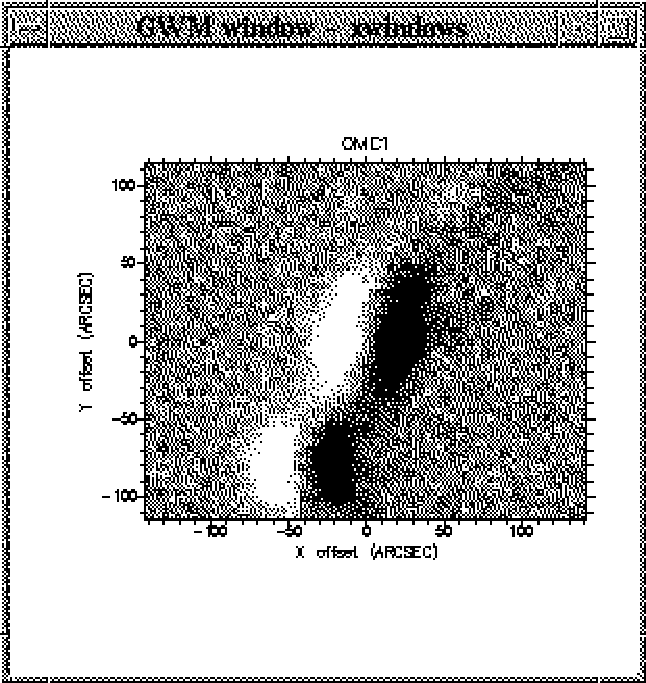
\includegraphics[height=80mm]{sc1_display2}
\end{center}

   If you would like to see only part of the image in more detail,
   you can choose a subset. In the jargon the data set is an
\htmlref{NDF}{glossndf}
   (or a base NDF), and a subset, superset etc.\ is an
\htmlref{NDF section:}{glossndfsection}

\begin{terminalv}
% display
IN - NDF to be displayed /@rxa_146m/ > rxa_146m(-50.:50.,-50.:50.)
MODE - Method to define the scaling limits /'scale'/ >
LOW - Low value for display /1.33531320095062/ >
HIGH - High value for display /9.29243278503418/ >
\end{terminalv}

   Note that the decimal points make this a subset in arc seconds from
   the centre. If you leave out the decimal points, the numbers would be
   counting the pixels from the bottom left.

\begin{center}
\leavevmode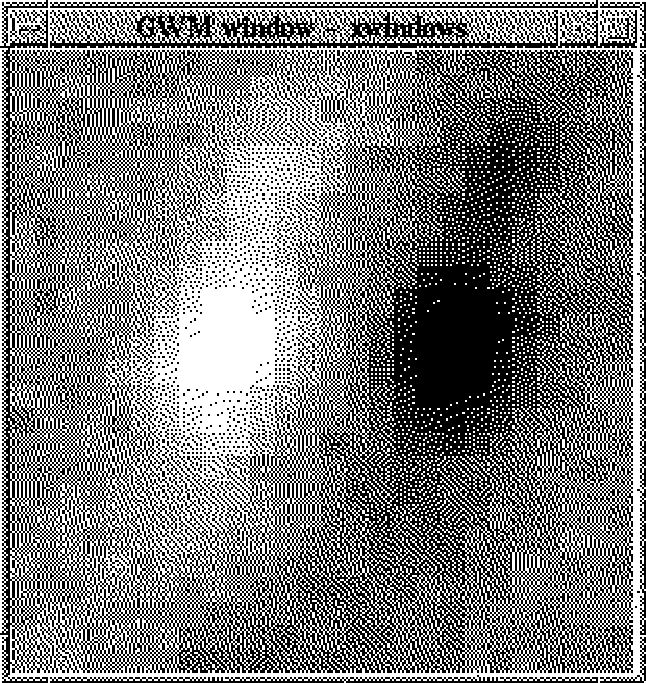
\includegraphics[height=80mm]{sc1_display3}
\end{center}

   Contour maps can be made using
\texttt{\xref{contour}{sun95}{CONTOUR}},
\texttt{\xref{turbocont}{sun239}{TURBOCONT}},
   or
\texttt{\xref{contover}{sun239}{CONTOVER}}.
   The latter is for overlaying a contour map on a grey-scale image.
   Alternatively, all or part of an image can be studied using
\texttt{\xref{inspect}{sun239}{INSPECT}}.

\subsection{\label{spikes2}\xlabel{spikes2}Alternative spike removal}

   If you have to interpolate within the row and have to ignore neighbour
   rows (e.g.\ if the other rows have a very different baseline level),
   you can use the Figaro routine
\texttt{\xref{clean}{sun86}{CLEAN}},
   which has separate options for interpolation within the row or within
   the column. \texttt{clean} also does the display itself and updates it
   as you zap pixels, and it allows you to change the grey scale and
   zoom factor. In \texttt{clean} set the size of the area to be deleted to
   1, using the command `N', and select the spikes with the cursor.
   Then the command `X' will replace the value in the bad pixel with an
   interpolation of the adjacent values in the same row. The command `S'
   can be used to change the display levels to allow spikes to be seen
   more clearly. Similarly, entire bad rows of data can be removed using
   the command `R', which substitutes the bad row with the interpolated
   values from the two adjacent rows.


\subsection{\label{base2}\xlabel{base2}Baseline correction}

   If you have to subtract linear baselines or different constants from
   each row of the map, you first use
\texttt{\xref{fitcheby}{sun140}{FITCHEBY}}
   once for each row, then you use
\texttt{\xref{evalfit}{sun140}{EVALFIT}}
   on the whole image to get a corresponding image containing the fitted
   baselines, and finally you subtract the baseline image from the
   original map with
\texttt{\xref{sub.}{sun95}{SUB}}
   In the fitting process we restrict \texttt{fitcheby} to the edges of
   the image, where both beams are off source. Here, we use a minimum
   offset of 120 arc seconds from the map centre.

   \texttt{fitcheby} can be run with or without graphics display. More,
   it can be run in an interactive loop, where you look at a plot and
   decide on the baseline intervals and polynomial order. You can also
   try a fit, look at it, and try something else. We do not demonstrate
   that mode here, since it would be too tedious to do that for each and
   every row of your map. Instead we run \texttt{fitcheby} without
   dialogue.

\begin{terminalv}
% fitcheby dialog=f device=xw order=1 comp=1 \
 mask1=\[-500,120\] mask2=\[-120,500\] accept in=rxa_146mc\(,1\)
% fitcheby device=xw \
 mask1=\[-500,120\] mask2=\[-120,500\] accept in=rxa_146mc\(,2\)
% fitcheby device=xw \
 mask1=\[-500,120\] mask2=\[-120,500\] accept in=rxa_146mc\(,3\)
...
% fitcheby device=xw \
 mask1=\[-500,120\] mask2=\[-120,500\] accept in=rxa_146mc\(,56\)
% fitcheby device=xw \
 mask1=\[-500,120\] mask2=\[-120,500\] accept in=rxa_146mc\(,57\)
\end{terminalv}

   Admittedly, you could write a Unix shell loop to do these 57 commands for
   you. The result of each fit is plotted. If you find that a fit went wrong
   you can repeat the fit for that row with more interaction. You also get
   screen output about the fit result:

\begin{terminalv}
Input NDF:  /tmp_mnt/home/hme/dump/rxa_146mc(1:71,24)
Varuse parameter:             F
No. of data points:          71
No. of mask intervals:        2
No. of valid data points:    12
Mask:
 -500.0000      -120.0000
  120.0000       500.0000
Actual abscissa range:
 -140.0000       140.0000
Order of polynomial: 1
Coefficients of series of Chebychev polynomials:
  10.28892     -0.1547112E-01
Degrees of freedom:          10
rms:                        0.1439584

Used component # 1 to store results.
\end{terminalv}

\begin{center}
\leavevmode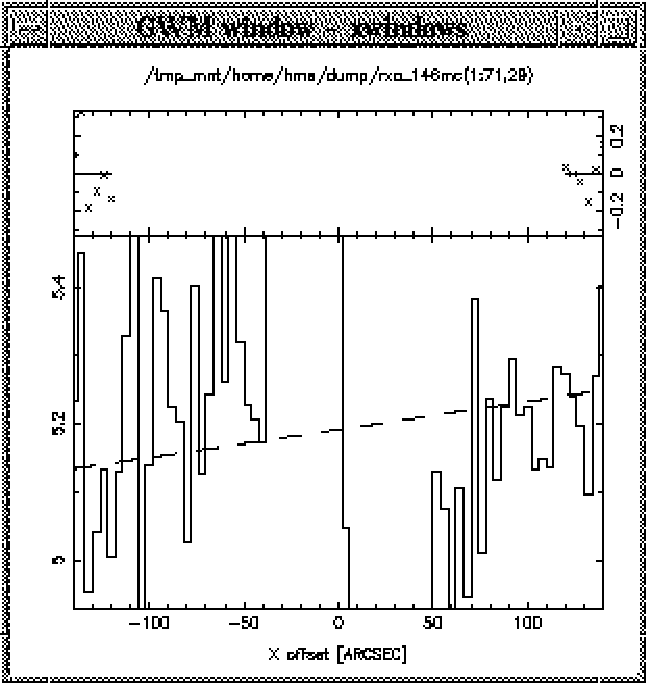
\includegraphics[height=80mm]{sc1_fitcheby}
\end{center}

   For each row the fit parameters have been stored along with the map
   in the data file. When all fits have been made, they can be evaluated
   and subtracted. You can also remove the fit results stored. At the
   end you can use
\texttt{\xref{editext}{sun140}{EDITEXT}}
   to remove the fit parameter storage.

\begin{terminalv}
% evalfit in=rxa_146mc out=baseline comp=1
% sub rxa_146mc baseline rxa_146mcs
% editext delete rxa_146mc
% editext delete rxa_146mcs
\end{terminalv}

\subsection{\label{beam}\xlabel{beam}Beam profile fit}

   In the absence of a routine to fit a beam map with a two-dimensional
   Gaussian function, we have to make do with one-dimensional fits
   along the central row and the central column. We can use
\texttt{\xref{fitgauss}{sun140}{FITGAUSS}}
   for this. A minor problem here is that the application normally
   assumes that it fits spectra and that spectra are rows. With the
\texttt{\xref{editext}{sun140}{EDITEXT}}
   commands we can convince it that spectra run along columns.

\begin{terminalv}
% fitgauss in=planet2\(,29\) comp=1 ncomp=1 cont=0 \
 centre=0 peak=20 fwhm=20 accept
...
Gauss components:
 #   centre pos.    peak height       FWHM       line integral
 1   -0.2451146       19.59172       19.04641       397.2078
+/-   0.3494171      0.7329797      0.8228144       14.86063
...
% editext delete planet2
% editext \"set specaxis 2\" planet2
% fitgauss in=planet2\(36,\) comp=1 ncomp=1 cont=0 \
 centre=0 peak=20 fwhm=20 accept
...
Gauss components:
 #   centre pos.    peak height       FWHM       line integral
 1   -0.9182005       20.02674       19.77099       421.4740
+/-   0.4838968      0.9995921       1.139490       21.03699
...
% editext delete planet2
\end{terminalv}

   The reason we fit both cuts through the source is that each fitted
   centre position tells us how far off centre the other cut passed. The
   deviation is small compared to the profile width of 19 arc seconds,
   and therefore does not matter for the peak value.


\subsection{\label{dbmem}\xlabel{dbmem}Maximum entropy restoration}

   One way to restore the
\htmlref{dual-beam maps}{glossdualbeam}
   to single-beam is by deconvolving the beam
   profile from the data, using the DBMEM software
\htmlref{(Richer 1991).}{refer}
   In this case the data output from
\texttt{\xref{jcmtextc}{sun132}{JCMTEXTC}}
   can be converted into the correct format for DBMEM using the
   programme
\texttt{\xref{map2mem}{sun132}{MAP2MEM}}:

\begin{terminalv}
% map2mem b1950=no input=rxa_146mcse output=rxa_146mcse binary=no accept
MAP2MEM - No pointing corrections applied
Coordinates are FK5 J2000.0
\end{terminalv}

   While the input file has of course a file name extension `.sdf', the
   output file has an extension of `.mem'. In fact there are two output
   files, the second having extension `.dbh'. Both are not binary but
   printable ASCII files. You should now proceed, following the
   documentation in the DBMEM User Guide
\htmlref{(Richer 1992).}{refer}

   DBMEM will not only restore single-beam maps from dual-beam maps, it
   will also transform from Az/El to RA/Dec and it will calibrate the
   map in Jansky rather than mV, and try to take care of the
\htmlref{error beam.}{glosserrorbeam}


\newpage
\appendix
\section{Appendix}

\subsection{\label{packs}\xlabel{packs}Software packages}

\begin{itemize}
\item Figaro \xref{(Starlink User Note 86)}{sun86}{}
   \begin{itemize}
   \item \xref{clean}{sun86}{CLEAN}: Patch bad lines and pixels
   \item \xref{copobj}{sun86}{COPOBJ}: Copy an HDS object
   \item \xref{creobj}{sun86}{CREOBJ}: Create an HDS object or file
   \item \xref{setobj}{sun86}{SETOBJ}: Assign value to an HDS object
   \item \xref{wdfits}{sun86}{WDFITS}: Write disk FITS
   \end{itemize}
\item IRAS90 \xref{(Starlink User Note 163)}{sun163}{}
   \begin{itemize}
   \item \xref{skygrid}{sun163}{SKYGRID}: Overlay sky coordinate grid
   \item \xref{skyphot}{sun163}{SKYPHOT}: Integrated flux density in region
   \item \xref{skywrite}{sun163}{SKYWRITE}: Write text at specified position
   \end{itemize}
\item JCMTDR \xref{(Starlink User Note 132)}{sun132}{}
   \begin{itemize}
   \item \xref{ae2rd1}{sun132}{AE2RD1}: Transform to RA/Dec tangent plane
   \item \xref{ae2rd2}{sun132}{AE2RD2}: Transform to RA/Dec tangent plane
   \item \xref{gsd\_print}{sun132}{GSD_PRINT}: ASCII dump of GSD binary file
   \item \xref{iras\_tag}{sun132}{IRAS_TAG}: Tag IRAS astrometry structure
   \item \xref{jcmtextc}{sun132}{JCMTEXTC}: Correct for atmospheric extinction
   \item \xref{jcmt\_help}{sun132}{JCMT_HELP}: JCMTDR on-line help
   \item \xref{jcmt\_xhelp}{sun132}{JCMT_XHELP}: JCMTDR Mosaic help browser
   \item \xref{makemap}{sun132}{MAKEMAP}: Convert GSD to NDF
   \item \xref{map2mem}{sun132}{MAP2MEM}: Export to DBMEM
   \item \xref{restore}{sun132}{RESTORE}: Deconvolve dual-beam map
   \end{itemize}
\item KAPPA \xref{(Starlink User Note 95)}{sun95}{}
   \begin{itemize}
   \item \xref{compave}{sun95}{COMPAVE}: Average neighbouring pixels
   \item \xref{compick}{sun95}{COMPICK}: Pick every n-th pixel
   \item \xref{contour}{sun95}{CONTOUR}: Contour an image
   \item \xref{contover}{sun239}{CONTOVER}: Overlay contours on display
   \item \xref{csub}{sun95}{CSUB}: Subtract scalar from data
   \item \xref{cmult}{sun95}{CMULT}: Multiply data by a scalar
   \item \xref{display}{sun95}{DISPLAY}: Display an image
   \item \xref{erase}{sun95}{ERASE}: Erase an HDS object
   \item \xref{gauss}{sun95}{GAUSMOOTH}: Smooth image with Gaussian filter
   \item \xref{gdset}{sun95}{GDSET}: Select graphics device
   \item \xref{idset}{sun239}{IDSET}: Select image-display device
   \item \xref{inspect}{sun239}{INSPECT}: Inspect image in a variety of ways
   \item \xref{lutgrey}{sun95}{LUTGREY}: Load grey scale lookup table
   \item \xref{lutneg}{sun95}{LUTNEG}: Load negative grey scale lookup table
   \item \xref{maths}{sun95}{MATHS}: Data sets in mathematical expressions
   \item \xref{ndfcopy}{sun95}{NDFCOPY}: Copy (section of) data set
   \item \xref{ndftrace}{sun95}{NDFTRACE}: Display attributes of a data set
   \item \xref{paldef}{sun95}{PALDEF}: Load the default palette
   \item \xref{palentry}{sun95}{PALENTRY}: Enter a colour into palette
   \item \xref{setunits}{sun95}{SETUNITS}: Set units string for a data set
   \item \xref{sqorst}{sun95}{SQORST}: Squash or stretch an image
   \item \xref{stats}{sun95}{STATS}: Simple statistics for a data set
   \item \xref{sub}{sun95}{SUB}: Subtract one data set from another
   \item \xref{transformer}{sun239}{TRANSFORMER}
   \item \xref{turbocont}{sun239}{TURBOCONT}: Contour an image quickly
   \item \xref{zaplin}{sun95}{ZAPLIN}: Patch regions in an image
   \end{itemize}
\item Specdre \xref{(Starlink User Note 140)}{sun140}{}
   \begin{itemize}
   \item \xref{editext}{sun140}{EDITEXT}: Edit the Specdre Extension
   \item \xref{evalfit}{sun140}{EVALFIT}: Evaluate fit results
   \item \xref{fitcheby}{sun140}{FITCHEBY}: Fit Chebyshev series to a spectrum
   \item \xref{fitgauss}{sun140}{FITGAUSS}: Fit Gauss profiles to a spectrum
   \end{itemize}
\item Utilities
   \begin{itemize}
   \item \xref{hdstrace}{sun102}{}: List an HDS structure
   \item \xref{psmerge}{sun164}{}: Merge and manipulate Encapsulated PostScript
   \item \xref{xdestroy}{sun130}{xdestroyCommand}: Delete a display window
   \item \xref{xmake}{sun130}{xmakeCommand}: Create a display window
   \end{itemize}
\end{itemize}

\subsection{\label{gloss}\xlabel{gloss}Glossary}

\begin{itemize}

\item\textbf{\label{glossbeammap}beam map}\\
   A map of a point source. The map
   then shows the beam of the telescope, which is also called the
   telescope characteristic or antenna pattern.

\item\textbf{\label{glosschopthrow}chop throw}\\
   The angular separation of the
   positive and negative beams in dual-beam observations.

\item\textbf{\label{glossdst}DST format}\\
   An older data format used only by
   Figaro. Since Figaro supports the NDF format used by other packages,
   NDF is the preferred format. Since JCMTDR uses the Figaro data access
   routines, the environment variable FIGARO\_FORMATS should be set to
   `ndf' or `ndf,dst' while using JCMTDR.

\item\textbf{\label{glossdualbeam}dual-beam}\\
   In dual-beam mode the telescope
   has in effect two beams of high
   sensitivity that point to adjacent directions on the sky. During data
   recording the signals from the two beams are subtracted from each
   other. For a point source a dual-beam map would show the source
   twice, once as an area of increased signal and once as an area of
   reduced signal.

\item\textbf{\label{glosserrorbeam}error beam}\\
   Apart from the main beam of the
   telescope, the size of which is determined by the diffraction from
   the main mirror size, there is a broader error beam caused by slight
   mis-alignments of the panels of the main mirror. The error beam
   cancels out partially in dual-beam observations if the chop throw is
   small compared to the size of the error beam. But if the error beam
   is not removed in that way, it causes complications in the
   calibration of extended-source maps from beam maps.

\item\textbf{\label{glossfits}FITS format}\\
   FITS is originally a simple flexible
   tape format and intended for transporting astronomical data from one
   place to the other, or from one software package to the other.

\item\textbf{\label{glossflux}flux density}\\
   The density part of the
   term relates to the fact that it is a spectral density, not a sky
   area density. The flux density is the amount of energy received per
   time interval, per antenna surface element, and per spectral
   bandwidth:

\[S_{\nu} = dE / (dt\, dA\, d\nu)\]

   In radio astronomy the unit of Jansky is used instead of an SI unit:

\[1\,{\rm Jy} = 10^{-26}\,{\rm W / (m^2\, Hz)}\]

   If you work out the flux density per unit solid angle, say in
   MJy/sr then you have calculated the intensity. An extended
   source has different intensity in different places. If you integrate
   the intensity over the solid angle of the source you find the source
   flux density. It is natural to calibrate a map in intensity units
   like MJy/sr. Calibrations in Jy/beam and Jy/pixel are confusing, but
   in fact nothing else.

\item\textbf{\label{glossgsd}GSD format}\\
   This is a JCMT-specific VAX-binary
   format used by the data recording software to store data.

\item\textbf{\label{glosshds}HDS format}\\
\xref{HDS}{sun92}{}
   is a low-level file format to
   store information in a hierarchical tree of structures. To the user
   of data reduction software HDS is important in the context of the NDF
   format and the structure trees that are extensions to NDF data sets.
   Also, the container files of NDFs are often referred to as HDS files,
   or as Starlink Data Files.

\item\textbf{\label{glosshpbw}HPBW}\\
   The half power beam width of the antenna
   characteristic. This is the angular diameter of the beam measured at
   the points where the beam profile is half the maximum value. An
   equivalent acronym used in other circumstances is FWHM, the full
   width at half maximum.

\item\textbf{\label{glossndf}NDF format}\\
\xref{NDF}{sun33}{}
   is an HDS-based format to store
   data sets of any dimension (spectra, images, cubes, etc.). The term
   NDF is used for the format, for the object library that provides
   access to such data, and also for the data sets themselves. An NDF
   (the data set) will often be the top-level structure in its container
   file, and hence identified with the file. But an NDF can be deeper
   down the hierarchy of HDS structures in the container file. Another
   important feature of NDFs is that they can have
\xref{named extensions}{sun33}{extensions}
   for use by certain applications. JCMTDR uses a `JCMT Extension' to its
   NDFs, which amongst other information contains another NDF with the
   local sidereal time for each pixel of the main NDF.
% The label does not exist in SUN/33, but seems
% a reasonable guess at a future xlabel.

\item\textbf{\label{glossndfsection}NDF section}\\
   In one of its interpretations
   the term `NDF' denotes a data set, an image, spectrum, cube etc.
   Most commands (not those from Figaro, mind) can work on a
\xref{section of an NDF}{sun33}{ndf_sections}
   rather than on the whole NDF. A section can be a subset, or a
   superset of an NDF, or a mixture between the two. The most common way
   to specify an NDF section is by giving coordinate ranges.
   \texttt{rxa\_146m(-50.:50.,-50.:50.)} uses the coordinates as stored
   in the axis structure of the NDF. This is because the decimal points
   are present. \texttt{rxa\_146m(25:,:25)} uses pixel numbers. Some of
   the range limits have been left out to use whatever is the end of the
   NDF.

\item\textbf{\label{glossnod2}NOD2}\\
   In this context, the precursor software to
   JCMTDR.

\item\textbf{\label{glossnullvalue}null value}\\
   When prompted for a parameter
   value you can specify the null value to say that there is no value,
   that the parameter should have no meaning. With most parameters that
   will cause an error in the application, but in some cases the
   application can make sense out of your statement that the parameter
   is to be unspecified. Say, if \texttt{istat} asks for the name of a log
   file, responding with the null value means `I don't want a log file.'

\item\textbf{\label{glossonthefly}on-the-fly}\\
   An on-the-fly map is taken while
   the source moves in horizontal coordinates. The telescope takes rows
   of the map by scanning through the azimuth offset from the source
   while keeping the elevation offset from the source constant.
   Successive rows are taken for different elevation offsets.

\item\textbf{\label{glossphotometric}photometric}\\
   The sky or a night is called
   photometric if conditions are stable enough to do photometry. These
   are better conditions than necessary for spectroscopy.

\item\textbf{\label{glossplanetmap}planet map}\\
   Synonymous with beam map.

\item\textbf{\label{glosssensset}sensitivity setting}\\
   The setting made during
   an observation for the detector signal in mV per radiation from the
   sky. The original data in your map (say just after \texttt{makemap}) are
   always between 0 and +10 mV. This scaling is achieved with the
   appropriate sensitivity setting. A sensitivity setting of 5 mV (10
   mV) means that 5 mV (10 mV) of `true' signal is scaled to 10 mV (10
   mV) in your raw data. Conversely, a raw data value of 1 mV (1 mV)
   corresponds to a true signal of 0.5 mV (1 mV).

\item\textbf{\label{glosssinglepoint}single-point photometry}\\
   Photometry done
   by pointing the telescope only at one position, rather than taking a
   small map of the source.

\item\textbf{\label{glosssdf}Starlink Data File}\\
   Another term for HDS container
   file. These files usually have a file name extension `.sdf', and they
   always contain a hierarchy of HDS structures, such as a data set in
   NDF format.

\end{itemize}


\subsection{\label{refer}\xlabel{refer}References}

Duncan et al., 1990, MNRAS 243, 126\\
Emerson, Klein \& Haslam, 1979, A\&A 76, 92\\
Griffin et al., 1986, Icarus  65, 244\\
Griffin \& Orton, 1993, Icarus 105, 537\\
Orton et al., 1986, Icarus 67, 289\\
Renka \& Cline, 1984, Rocky Mountain J. Math 14, 223\\
Richer, 1991, MNRAS 254, 165\\
Richer, 1992, DBMEM User's Guide, MRAO, Cambridge\\
Sandell, 1994, MNRAS 271, 75\\
Stevens \& Robson, 1994, MNRAS 270, L75\\

\xref{Starlink User Note 33}{sun33}{}: NDF -- Routines for
   accessing the Extensible N-Dimensional Data Format -- Programmer's
   manual\\
\xref{Starlink User Note 42}{sun42}{}: DAOPHOT -- Stellar
   photometry package\\
\xref{Starlink User Note 86}{sun86}{}: FIGARO -- A general data
   reduction system\\
\xref{Starlink User Note 92}{sun92}{}: HDS -- Hierarchical Data
   System -- Programmer's manual\\
\xref{Starlink User Note 95}{sun95}{}: KAPPA -- Kernel application
   package\\
\xref{Starlink User Note 102}{sun102}{}: HDSTRACE -- Listing HDS
   data files\\
\xref{Starlink User Note 130}{sun130}{}: GWM -- X graphics window
   manager\\
\xref{Starlink User Note 132}{sun132}{}: JCMTDR -- Applications
   for reducing JCMT data\\
\xref{Starlink User Note 140}{sun140}{}: SPECDRE -- Spectroscopy
   data reduction\\
\xref{Starlink User Note 141}{sun141}{}: Starman -- A stellar
   photometry package\\
\xref{Starlink User Note 163}{sun163}{}: IRAS90 -- IRAS Survey and
   PO data analysis package -- Reference guide\\
\xref{Starlink User Note 164}{sun164}{}: PSMERGE -- Encapsulated
   PostScript handling utility\\
\xref{Starlink User Note 175}{sun175}{}: MOSAIC -- A hypertext
   help system\\


\end{document}
